\documentclass{sig-alternate}
\usepackage{etoolbox}
\makeatletter
\patchcmd{\maketitle}{\@copyrightspace}{}{}{}
\makeatother

\usepackage[caption=false]{subfig}
\usepackage{verbatimbox}



\begin{document}

\title{Supervised Learning}
\subtitle{Writeup for Assignment 01 - CS 6741}

\author{
\alignauthor
Magahet Mendiola
}
\date{}

\maketitle
\begin{abstract}
An analysis of two machine learning classification problems, including an evaluation of various learning algorithms' performance and behavior on the datasets.
\end{abstract}
 

%a description of your classification problems, and why you feel that they are interesting. Think hard about this. To be at all interesting the problems should be non-trivial on the one hand, but capable of admitting comparisons and analysis of the various algorithms on the other.

\section{Data}

Two classification datasets have been chosen based on the following criteria: Each dataset includes a minimum of 3,000 instances to insure sufficient data to evaluate each learning algorithm. Test sets were created by taking a uniform random sample of 33\% of the original instances without replacement. The remaining 66\% were then used as a training superset. Smaller subsets were pulled from this partition as needed.


\section{Classification - Mushrooms}

The first dataset is titled, Mushroom \cite{Bache+Lichman:2013} and was chosen from the UCI ML Repository. The classification task for this dataset is to determine whether a given mushroom is edible or poisonous based on the specimen's physical attributes. There are 22 recorded attributes which describe the physical appearance and olfactory perception of each sample. A full description of attributes can be found at http://archive.ics.uci.edu/ml/datasets/Mushroom.

This dataset allows for experimentation of various learning algorithms against attributes with only discrete values. The recorded attributes also require minimal domain knowledge to interpret, which reduces complexity in conceptualizing relationships and evaluating each learner's behavior.


\subsection{Attribute characteristics}

By examining the value distributions as seen in Figure~\ref{ag-data-viz}, we first observe that the two classifications are fairly evenly distributed (48\% edible, 52\% poisonous). This allows for the evaluation of learning algorithm accuracy based on the percentage of classification mistakes made by the model on our test set. This metric will not be unduly weighted by a greater occurrence of one of the classes. It is worth considering the use cases for such a model though. For example, if it were used to decide whether to serve a given mushroom to a class full of students, we would prefer a hypothesis that identified all the poisonous mushrooms, even if it meant misclassifying a number of edible samples. To be more precise, we would be most concerned with the recall of the poison class to insure we identify a high percentage of those mushrooms that are in fact poisonous. For the purpose of this first classification task, we will focus on the simple metric of classification error.

Each attribute includes a finite and limited set of values (min: 2, max:12). This indicates that information gain would provide a suitable metric for decision tree attribute selection, as the variance in value ranges is not significant and, similar to our reasoning for class distribution, we will not need to account for attributes with greater than average ranges of values.

With all the attributes taking discrete (nominal) values, learning algorithm options will be somewhat constrained. For example, neural network network input nodes will need to be setup for each attribute value pair; separating them into binary attributes for each value. The behavior of k-nn will also be constrained. Distance metrics for such attributes will either be simplistic (testing for exact matches) or less intuitive than measuring euclidean distance.

\begin{figure}[!htbp]
    \centering
    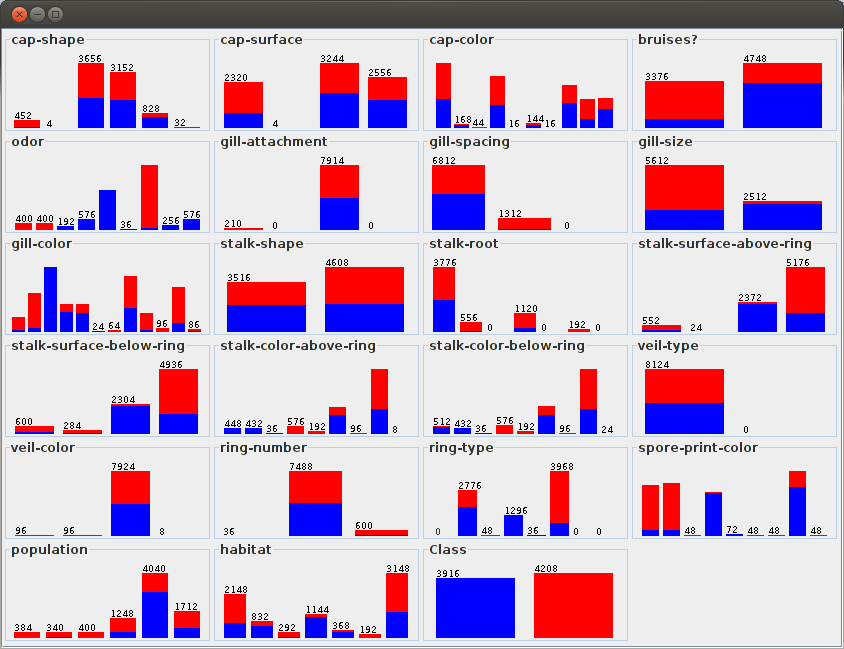
\includegraphics[width=3in]{data/agaricus-lepiota/ag-data-viz.png}
    \caption{mushroom attribute distribution and classification \label{ag-data-viz}}
\end{figure} 

We can observe, visually, that a number of attributes provide clear separability between the target classes. This supports the intuition that our attributes do have some functional relationship to the classes. In fact, it appears from the figure that the odor attribute, by itself, could provide a fairly clear indicator of how a sample should be classified. Spore-print-color appears to provide decent class separation as well. We can predict that these attributes will be heavily weighted during the attribute selection or weighting process.

\subsection{Algorithm Evaluations}
%the training and testing error rates you obtained running the various learning algorithms on your problems. At the very least you should include graphs that show performance on both training and test data as a function of training size (note that this implies that you need to design a classification problem that has more than a trivial amount of data) and--for the algorithms that are iterative--training times.

Each leaning algorithm has been applied to the training data with the same procedure. As described earlier, a subset of data was partitioned and preserved as a testing set. The remaining instances were then sampled from to create smaller training sets for use in evaluating each learning algorithms' performance and behavior.


\subsubsection{Learning Curves}

Evaluation began by choosing conservative starting values for each learners' parameters. Then each learner was trained against a range of training set sizes between 10 and 2000 instances (increments of 10). After each training phase, the original test data (1/3 of the original dataset) was used to evaluate the learner's performance. In this case, classification error was used as the performance metric. The plot in Figure~\ref{ag-error} shows each learning algorithm's results.

A number of assumptions are made for this initial evaluation. The goal of the exercise being to obtain a general intuition regarding each algorithms' performance, and not to present ideal conditions. Further parameter changes are discussed in subsequent sections of this analysis. The following describes the initial conditions for each learning algorithm.

\begin{description}
    \item[Decision Tree] Weka's open source version of the C4.5 algorithm (J48) was chosen, which uses normalized information gain ratio to select attributes. Post-pruning was done with a minimum leaf size of 2 instances a confidence factor of 0.25.
    \item[Boosting] It would be beneficial to compare our single iteration C4.5 to the same learner with boosting enable. Unfortunately, that was not possible with this dataset. As can be observed in the learning curve plots below, that the training error for C4.5 was negligible. This caused the boosting algorithm to compute a zero classification error tree in most cases. This resulted in the boosting process returning after a single decision tree was built. This behavior persisted even with more aggressive post-pruning parameters. In order to evaluate boosting, a weaker learner was chosen in place of C4.5. Boosting was performed on a decision stump learner, which is a simplistic decision tree algorithm that creates a single node/attribute tree based on the attribute with the best information gain.
    \item[Neural Network] A multilayer perceptron network was used with one hidden layer using a sigmoid activation function. Input nodes were created for each attribute/value pair, and 63 hidden nodes were used, which is the number of input nodes plus the number of output nodes divided by two. The algorithm performs gradient decent to adjust weights, and includes both a learning rate and a momentum factor to slow down and smooth weight changes. For this test, both terms are held static (learning rate = 0.3, momentum = 0.2).
    \item[k-NN] For the initial experiment, the nearest neighbor algorithm was set to k = 1. This matches the single closest instance from the training set to determine a classification. The distance metric used is euclidean distance. The plot titles for k-NN are IBk, which is the Weka implementation of the algorithm. 
    \item[SVM] SVM was run initially with a linear kernel (polynomial with degree 1). Both polynomial and radial basis function kernels are evaluated later. The plot title for SVM is SMO, which is Weka's implementation of SVM.
\end{description}

\begin{figure}[!htbp]
    \centering
    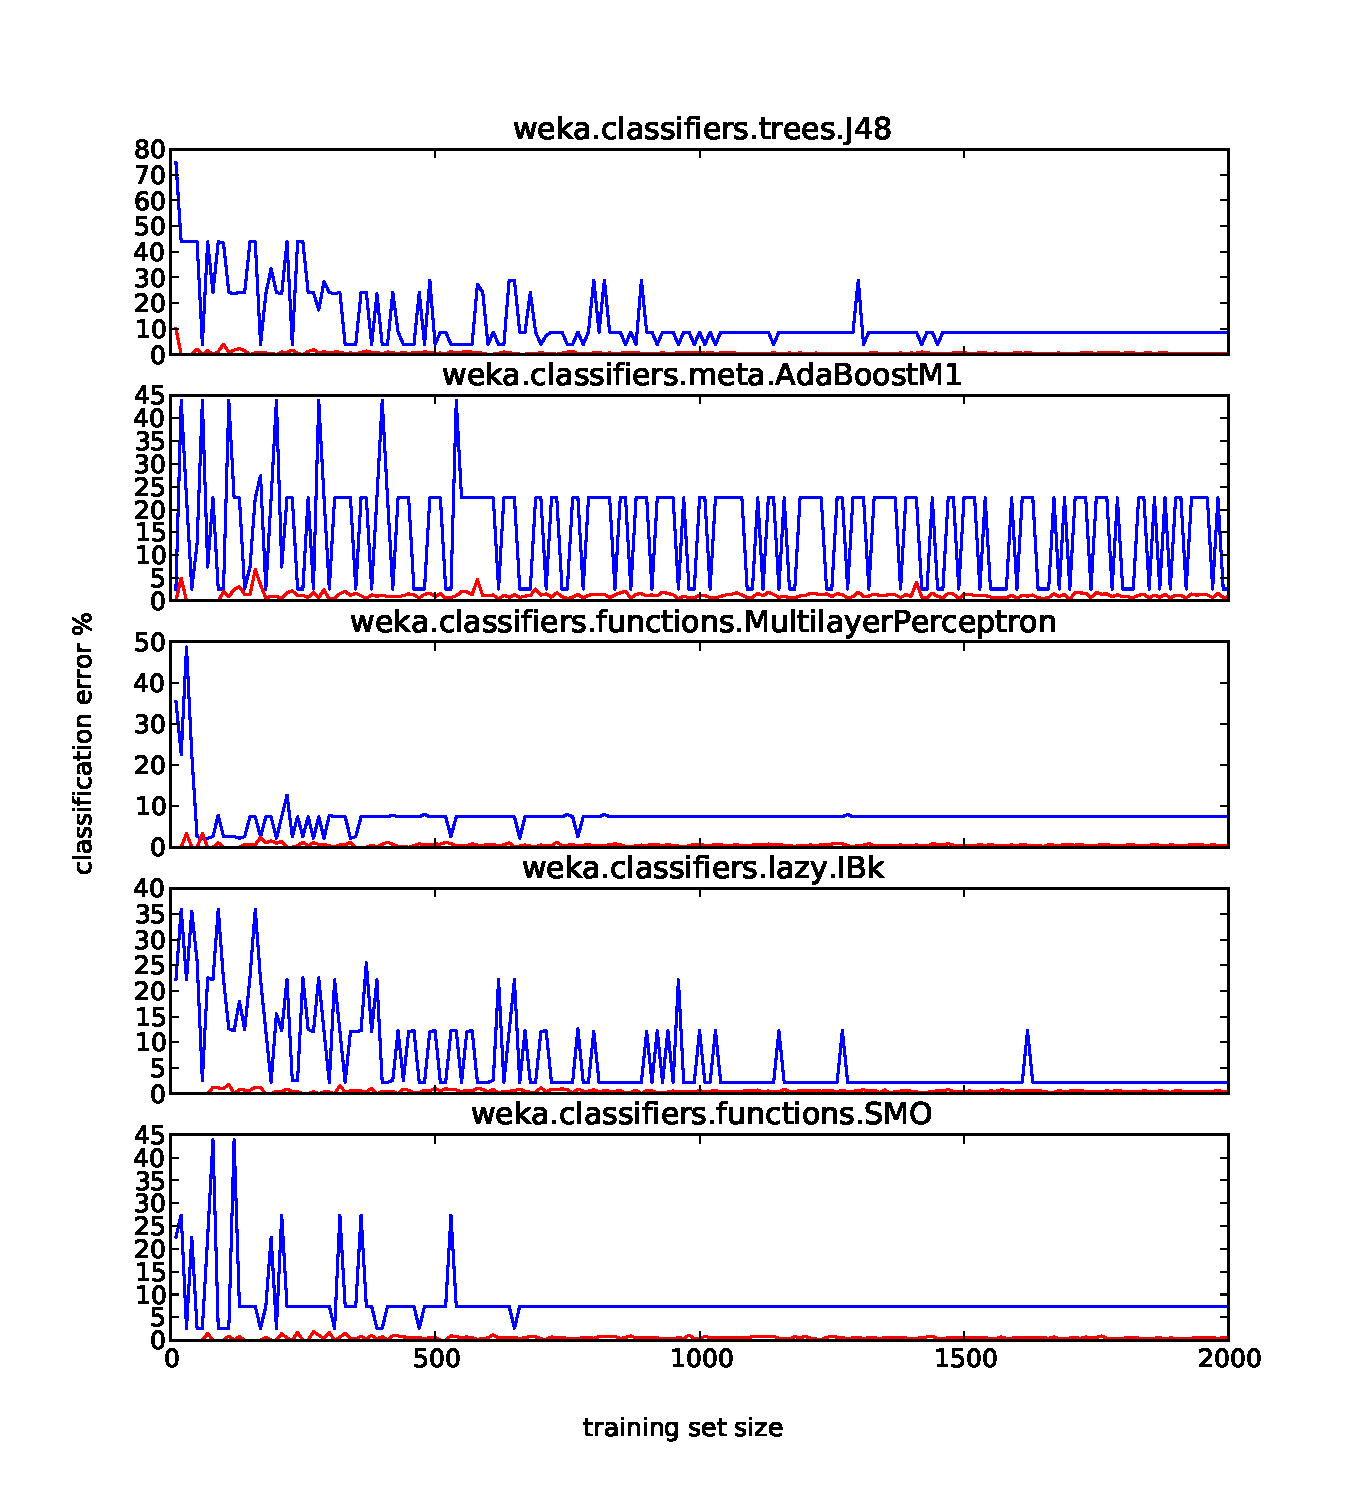
\includegraphics[width=3in]{data/agaricus-lepiota/learning-curve-10to2000/stacked-test-error.pdf}
    \caption{Mushroom - Classification Error by Training Size \label{ag-error}}
\end{figure} 

The results show training error (red lines) for every learner remain below 10\%. In all cases, except decision trees, this error was never higher than 5\% even with only 10 samples to train from. This indicates that our learners were able to converge to a hypothesis that fit the training data very well for small sample sizes. The overall dataset seems to have a little variance and each learner is able to closely model the training data.

The testing error plots (blue lines) also exhibit low error for most learners, with the exception of boosting. As expected, smaller training sample sizes show higher misclassification rates. The error rates quickly drop to below 10\% for training sets around 1,000 samples. Comparing each learner, we see that our perceptron network was able to reach this low level of classification error with the smallest number of training examples (about 100). However, the runtime plot in Figure~\ref{ag-runtime} shows this learner was the slowest to train by an order of magnitude. Depending on the use case, a trade-off can be made for which learner to implement based on the amount of training data available and the time allotted for training.

Another interesting result can be seen in our boosting algorithm, which struggled to reach the same level of classification error as the others. The intuition for this is that as there are certain attributes with much greater performance metric results which unduly influenced the ability of the weak learner to find suitable attributes other than those with the most influence on the classification.


\subsubsection{Training Times}

The elapsed time required for each learner to consume the training set has been plotting in Figure~\ref{ag-runtime}. Results from this data indicate that C4.5 performed well in this regard. Training time for decision trees appeared to run two orders of magnitude faster than our neural network, and one order greater than SVM. The perceptron network seemed to grow linearly and remained far above any other learner. The one surprise in the results was k-NN, which seemed to take longer to train than decision trees. This may be due to the preprocessing, such as sorting, of samples to prepare them for faster distance measurements.


\begin{figure}[!htbp]
    \centering
    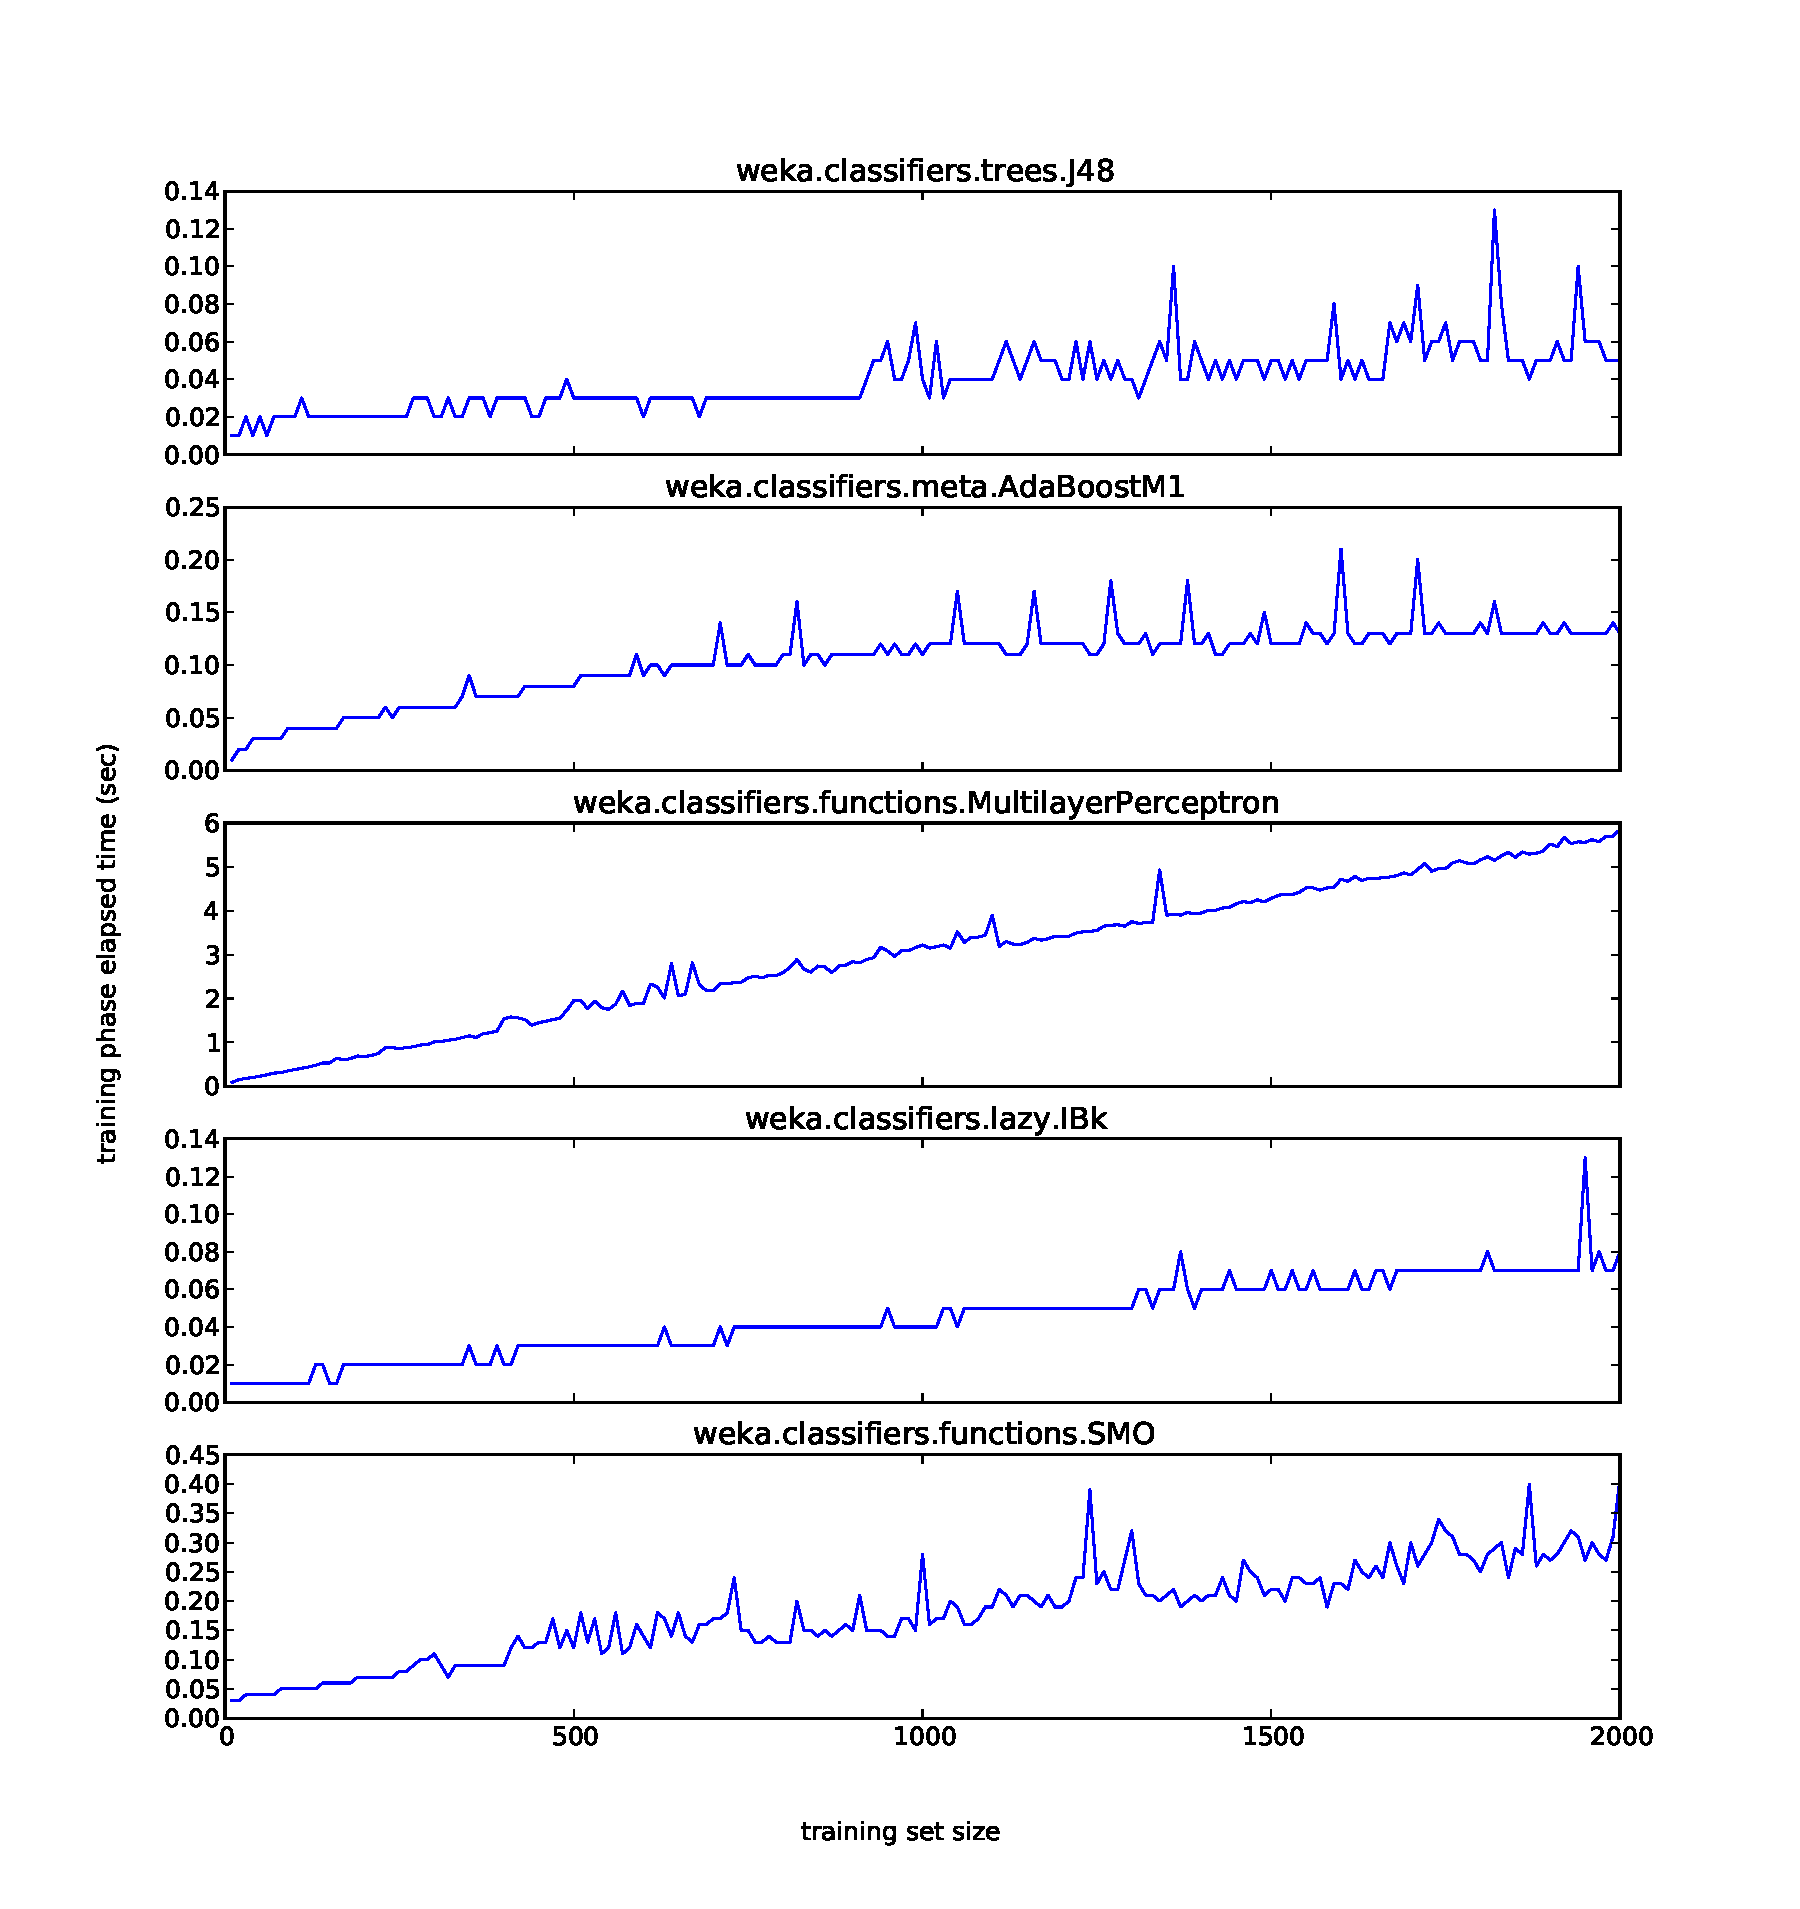
\includegraphics[width=3in]{data/agaricus-lepiota/learning-curve-10to2000/runtime.pdf}
    \caption{Mushroom - Training Time by Training Size \label{ag-runtime}}
\end{figure} 


\subsection{Decision Trees}
%Decision Trees. For the decision tree, you should implement or steal a decision tree algorithm. Be sure to use some form of pruning. You are not required to use information gain (for example, there is something called the GINI index that is sometimes used) to split attributes, but you should describe whatever it is that you do use.

Further experimentation into the decision tree learner was performed on subsets of the original data. As before, 1/3 of the data was partitioned for testing. The training set was then taken as 1,000 instances from the remaining set.

As a baseline, the learner was run with initial settings, which included post-pruning with a 0.25 confidence factor and a minimum leaf size of 2 instances. These settings produced the tree in Figure~\ref{dt-c025}. This tree produced no training classification error and 12\% error on the test set. The majority of training instances were classified based on two attributes, odor and stalk-shape.

\small
\begin{verbbox}
odor = a: e (69.0)
odor = l: e (77.0)
odor = c: p (37.0)
odor = y: p (6.0)
odor = f: p (234.0)
odor = m: e (0.0)
odor = n
|   stalk-shape = e
|   |   habitat = g: p (3.0)
|   |   habitat = l
|   |   |   bruises? = t: p (3.0)
|   |   |   bruises? = f: e (4.0)
|   |   habitat = m: p (4.0)
|   |   habitat = p: e (0.0)
|   |   habitat = u: e (16.0)
|   |   habitat = w: e (18.0)
|   |   habitat = d
|   |   |   stalk-surface-above-ring = f: p (0.0)
|   |   |   stalk-surface-above-ring = y: p (0.0)
|   |   |   stalk-surface-above-ring = k: p (4.0)
|   |   |   stalk-surface-above-ring = s: e (4.0)
|   stalk-shape = t: e (468.0)
odor = p: p (51.0)
odor = s: p (2.0)

Number of Leaves  :     20

Size of the tree :  25
\end{verbbox}
\normalsize

\begin{figure}[!htbp]
    \centering
    \theverbbox
    \caption{c4.5 decision tree with 0.25 confidence interval \label{dt-c025}}
\end{figure}


The discrepancy in training and testing error indicates that the learner may be overfitting the training data. This is further supported by the small number of instances categorized by deeper leaves. To try to archive better generalize, the same process was repeated with more aggressive post-pruning parameters. The results of setting the confidence factor to 0.01 is shown in Figure~\ref{dt-c001}.

\small
\begin{verbbox}
odor = a: e (69.0)
odor = l: e (77.0)
odor = c: p (37.0)
odor = y: p (6.0)
odor = f: p (234.0)
odor = m: e (0.0)
odor = n: e (524.0/14.0)
odor = p: p (51.0)
odor = s: p (2.0)

Number of Leaves  :     9

Size of the tree :  10
\end{verbbox}
\normalsize

\begin{figure}[!htbp]
    \centering
    \theverbbox
    \caption{c4.5 decision tree with 0.01 confidence interval \label{dt-c001}}
\end{figure}

Although a negligible number of instances were miscategorized from the training set, the classification error on the test set dropped to 4\%. The resulting tree is made up of a single attribute node with nine leaves. This confirms the initial hypothesis that overfitting was occurring with the starting parameters. We can also see that, as expected, the odor attribute does exert a great deal of influence on correct classification. To validate this further, Weka's attribute evaluator tool was used to calculate the information gain for this attribute, which came out to 0.83. This confirms further the strength of this attribute in classification.

We should note that adjusting the post-pruning parameters further would have no effect on the tree, as there is only a single node and the tree cannot be pruned further. When run with no post-pruning performed, the same tree is produced as with the initial settings.



\subsection{Neural networks}
%For the neural network you should implement or steal your favorite kind of network and training algorithm. You may use networks of nodes with as many layers as you like and any activation function you see fit.

The neural network learner was able to reach a low classification error with a very small training set (around 100 instances). To evaluate this learner in greater detail, the experiment was repeated with the following conditions:

\begin{itemize}
    \item training set size was held at 1,000 instances
    \item learning rate (how much weights are changed each iteration), were varied from 0.1 to 3.0
    \item training iterations are varied between 10 and 1,000 (by 10s)
    \item number of hidden nodes are varied manually
\end{itemize}

The results from varying the learning rate and training iterations is displayed in Figures~\ref{ag-nn-ti}~and~\ref{ag-nn-lr}. These plots show variance in the classification error for training iterations and learning rate. However, there is no discernible trend that would indicate better performance of the learner with a specific parameter value.

From examination of the attribute value distribution, and interpreting the results from the decision tree algorithm, it can be hypothesized that very few attributes have an influence on classification. Furthermore, there seems to be a direct relationship between those attributes and the class. This leads to the intuition that hidden layers in our neural network may be superfluous. It turns out, through repeating the experiment with decreasing numbers of hidden nodes, that classification error does not increase considerably. When a network with no hidden layer is trained, the error actually dropped from 7.7\% to 7.6\%. The significant advantage to this simplified network is the training time difference. The new network, with 63 fewer nodes, was able to train on the dataset in 1\% of the original time.

It is also interesting that the attributes identified by the decision tree algorithm as being the most relevant show the highest weights on the output nodes. This can be seen in the subset of weight outputs in Figure~\ref{ag-nn-weights}.


\begin{figure}[!htbp]
    \centering
    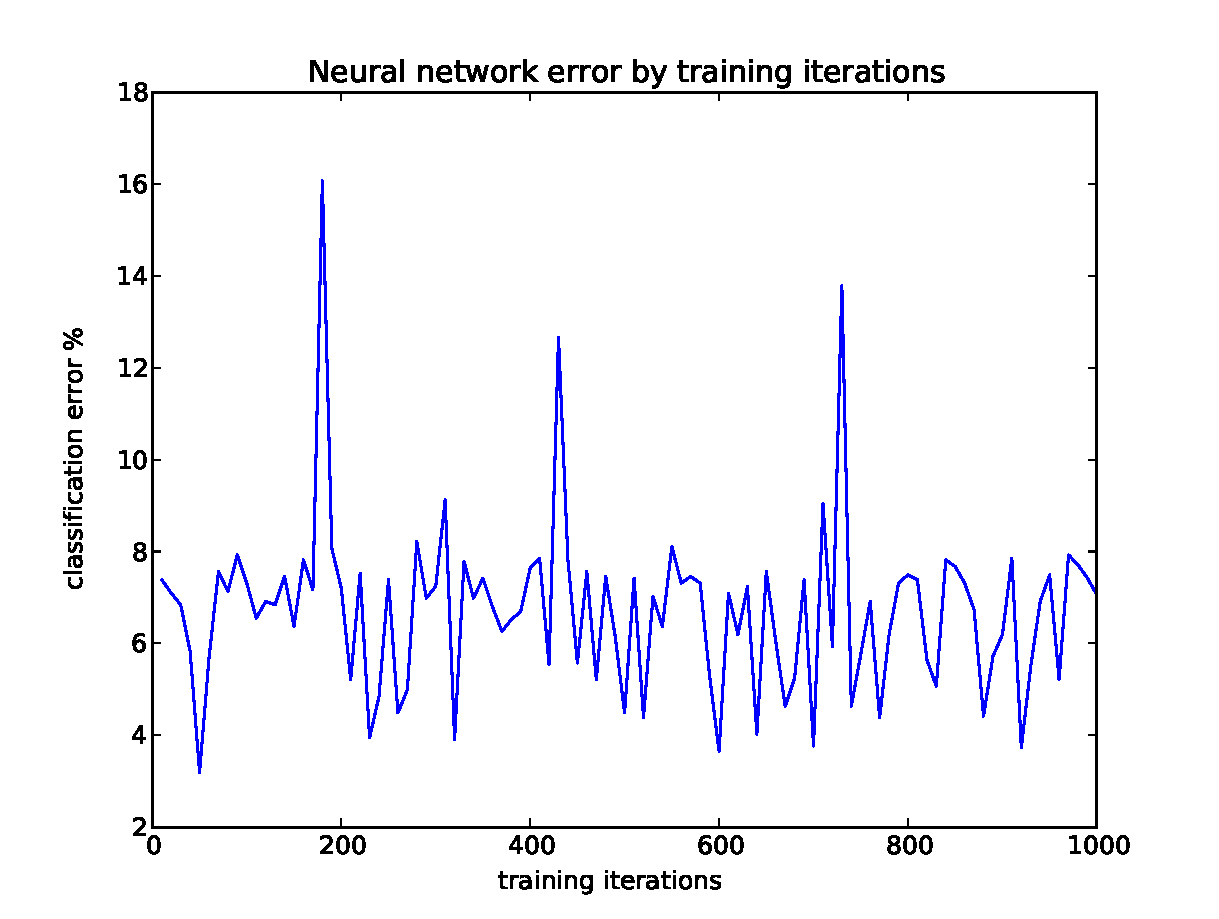
\includegraphics[width=3in]{data/agaricus-lepiota/perceptron/training-iterations.pdf}
    \caption{mushroom - neural network error by training iterations \label{ag-nn-ti}}
\end{figure} 

\begin{figure}[!htbp]
    \centering
    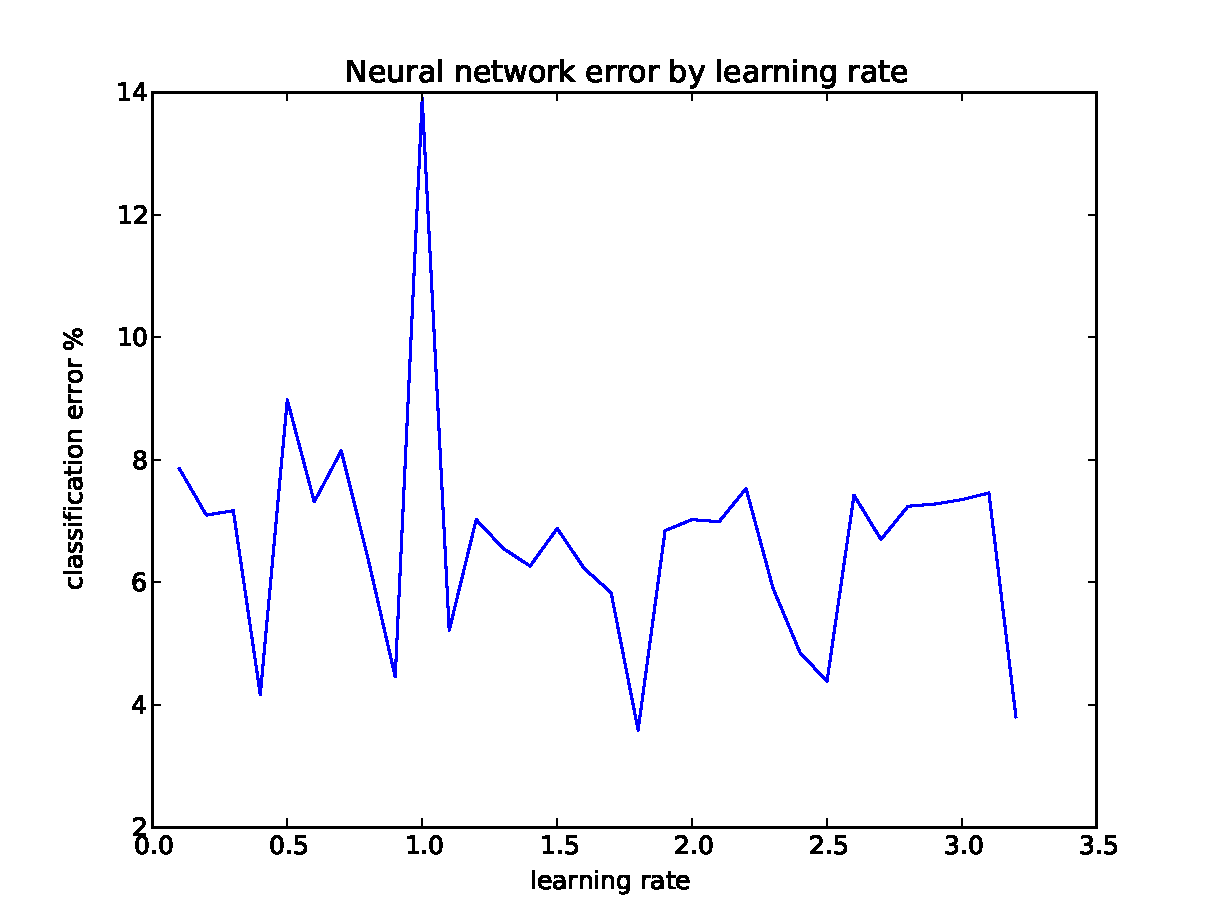
\includegraphics[width=3in]{data/agaricus-lepiota/perceptron/learning-rate.pdf}
    \caption{mushroom - neural network error by learning rate \label{ag-nn-lr}}
\end{figure} 

\small
\begin{verbbox}
Attrib cap-color=u    0.32909165328321105
Attrib cap-color=e    0.27084200618784854
Attrib cap-color=w    -0.6781600170313064
Attrib cap-color=y    -0.0944215007903694
Attrib bruises?    -0.20164966240021834
Attrib odor=a    1.9591467769018915
Attrib odor=l    2.163249089101404
Attrib odor=c    -1.938000290279853
Attrib odor=y    -0.7210176961657636
Attrib odor=f    -1.4655475615783258
Attrib odor=m    -0.0022502391144373773
Attrib odor=n    2.249162579023187
Attrib odor=p    -2.08204828811813
Attrib odor=s    -0.2329200532370795
Attrib gill-attachment=a    -0.016241324327899875
Attrib gill-attachment=d    0.0167616393841718
Attrib gill-attachment=f    0.04167201385764717
Attrib gill-attachment=n    -0.023866806192559844
Attrib gill-spacing=c    -0.8456690489234284
Attrib gill-spacing=w    0.8125552864255976
\end{verbbox}
\normalsize

\begin{figure}[!htbp]
    \centering
    \theverbbox
    \caption{neural network sample output node weights \label{ag-nn-weights}}
\end{figure}


\subsection{Boosting}
%Implement a boosted version of your decision trees. As before, you will want to use some form of pruning, but presumably because you're using boosting you can afford to be much more aggressive about your pruning.

As noted earlier, the boosting algorithm continued to oscillate between high and low classification errors as the training set size increased. A follow up test was performed to see if differing boosting iterations would have an effect on the overall error. The results are shown in Figure~\ref{ag-boost-iter}. This plot shows that after around 50 training iterations, boosting began producing models with higher classification error on the test set. This indicates that overfitting begins to occur and the model is no longer able to generalize well.

\begin{figure}[!htbp]
    \centering
    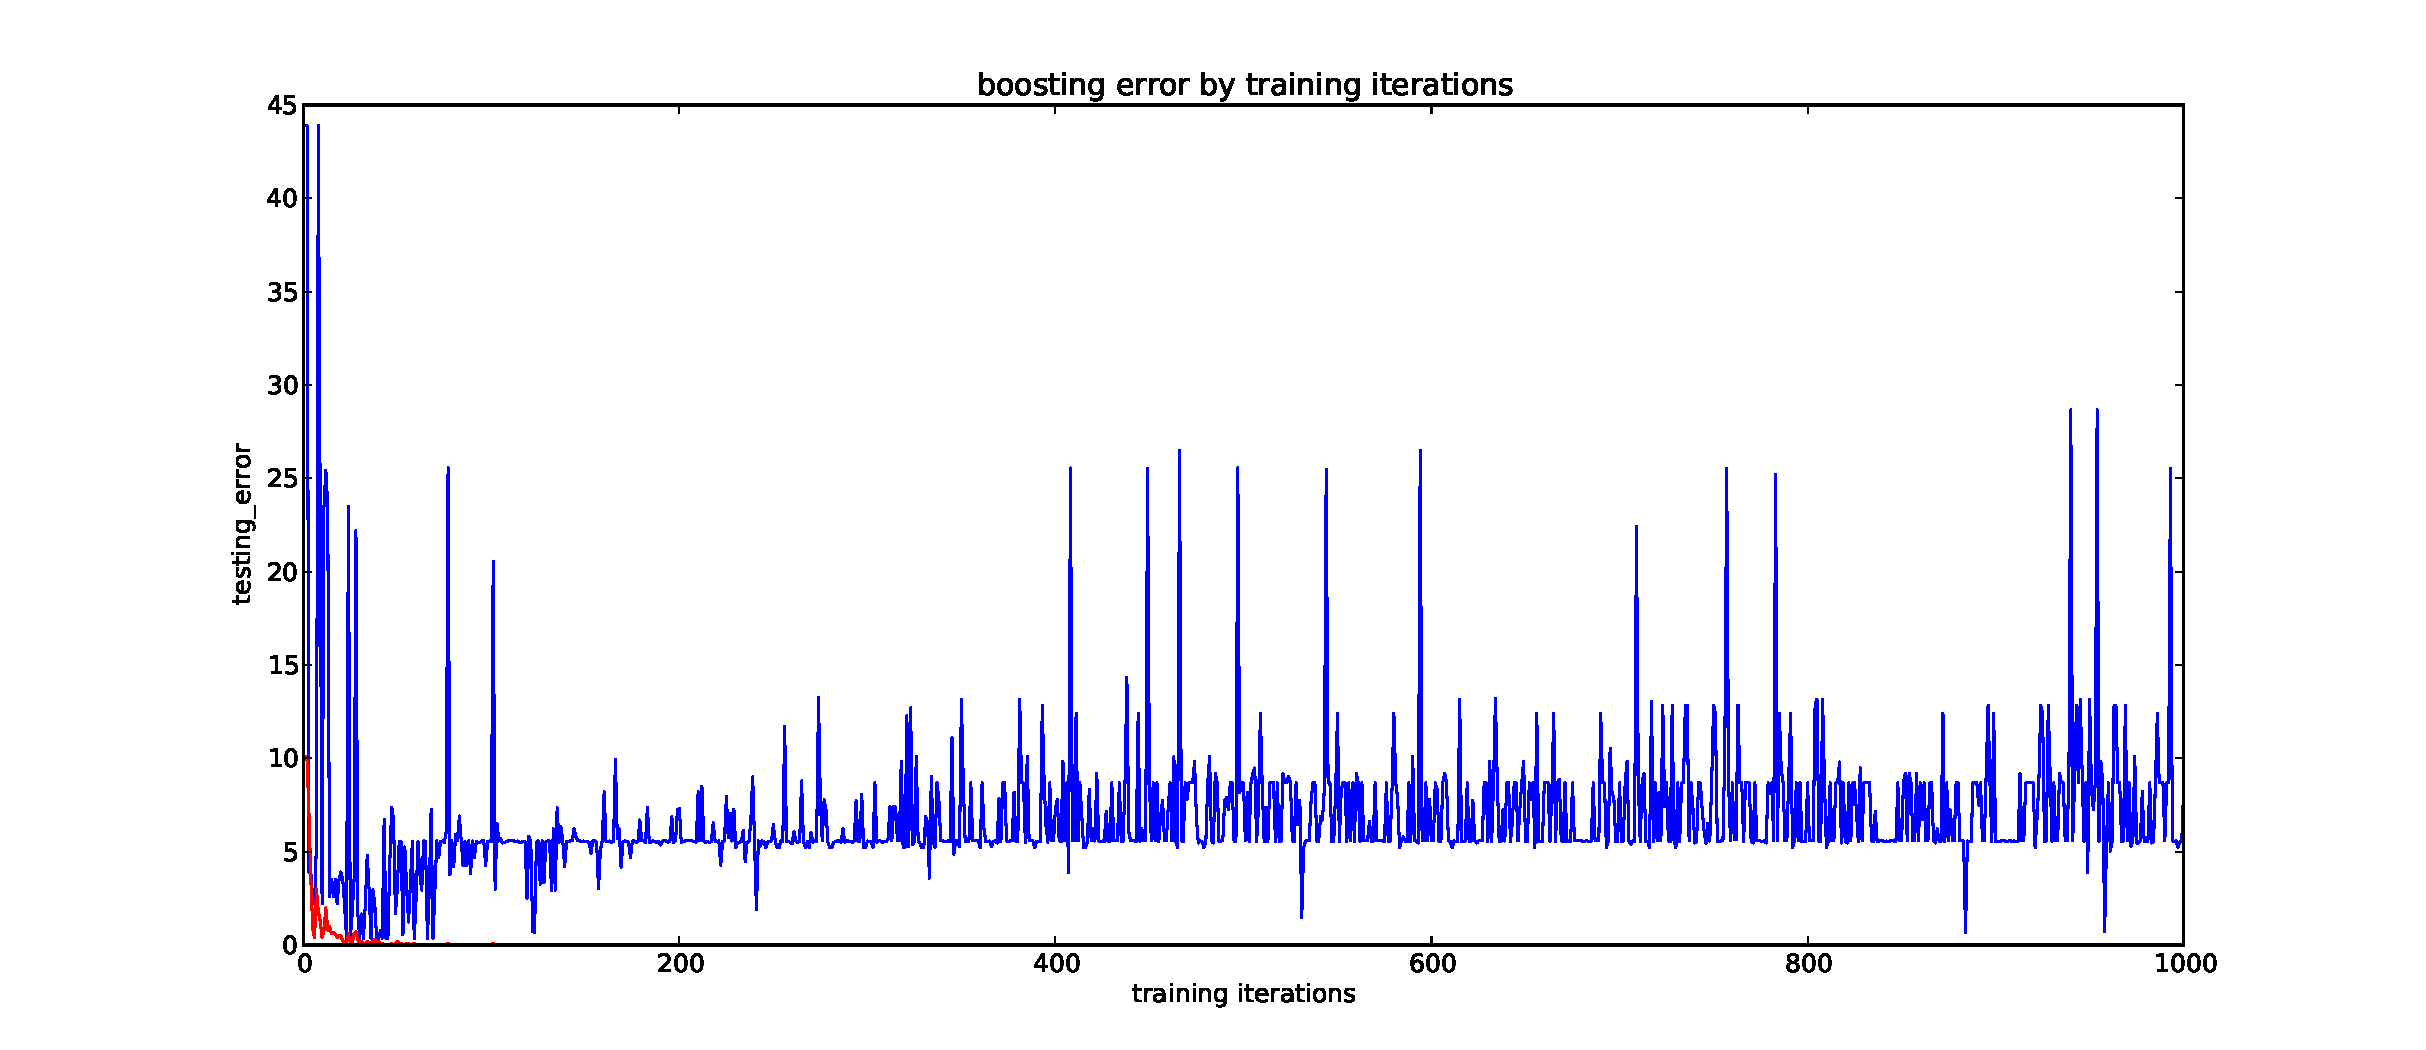
\includegraphics[width=3in]{data/agaricus-lepiota/boosting/training-iterations.pdf}
    \caption{Mushroom - error by boosting iterations \label{ag-boost-iter}}
\end{figure} 

An examination of the boosting behavior shows that the odor attribute was chosen by the weak learner (decision stump) for many of the boosting iterations. Each time the instance weight distribution caused the learner to select a different attribute, the odor attribute was again chosen during the subsequent iteration.


\subsection{Support Vector Machines}
%You should implement (for sufficently loose definitions of implement including download) SVMs. This should be done in such a way that you can swap out kernel functions. I'd like to see at least two.

The SVM performance in the initial experiment performed well in regards to quickly converging to low classification error with just over 500 samples. This learner also performed quite consistently at the low test error rate as more training data was added. The SVM training times were the second highest, being consistently double to triple that of the other eager learners. It was still significantly faster than the neural network. Even after dropping the 63 nodes in the hidden layer, the neural network was still significantly slower than SVM at the same training set size.

Follow up experiments were performed to see how changes to the SVM kernel would affect it's performance. It can be seen from Figure~\ref{ag-svm-poly} that using a polynomial kernel function with degree 6 produced the smallest classification error (2\%), which is significantly lower than that achieved by the linear kernel (7\%).

\begin{figure}[!htbp]
    \centering
    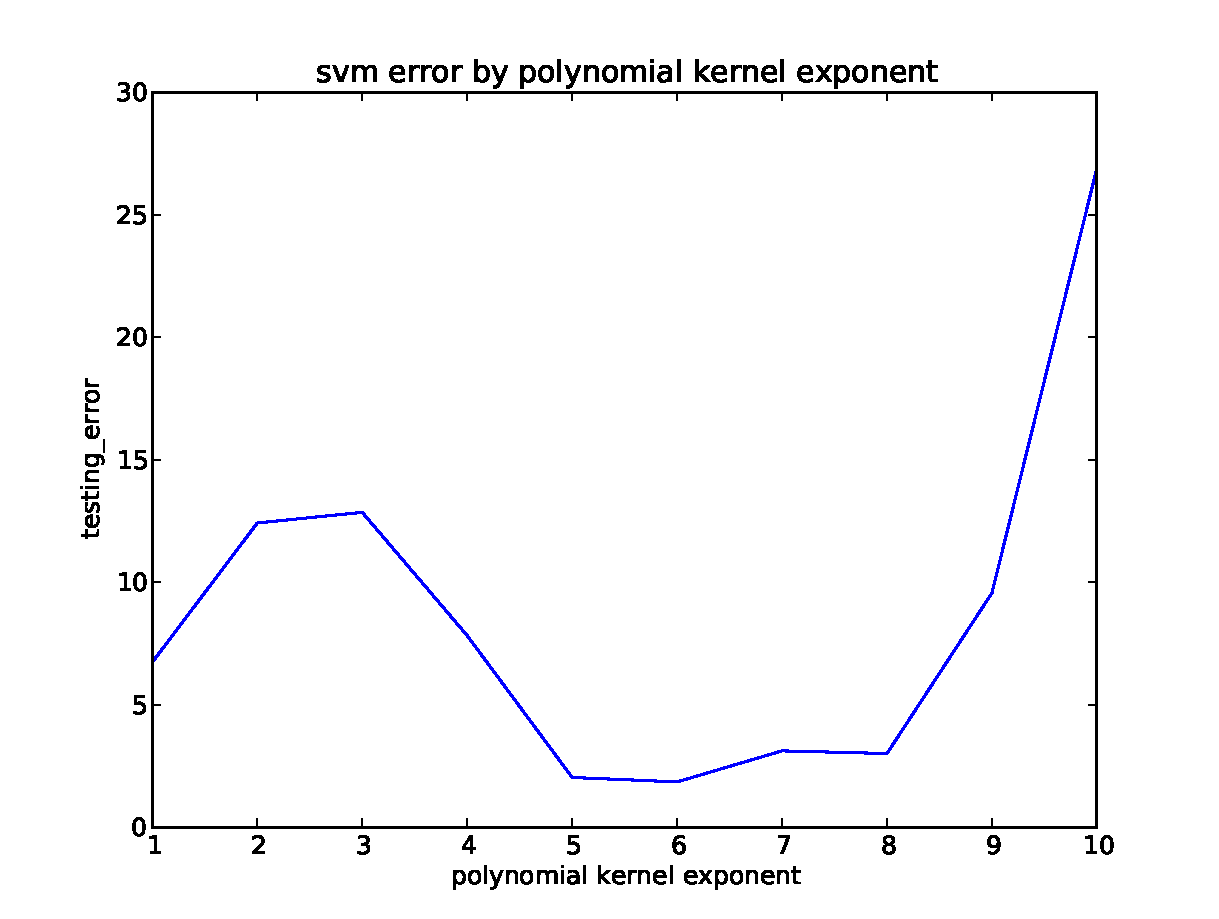
\includegraphics[width=3in]{data/agaricus-lepiota/svm/polynomial.pdf}
    \caption{Mushroom - error by svm polynomial kernel exponent \label{ag-svm-poly}}
\end{figure} 

The SVM kernel was then changed to a radial basis function to evaluate it's behavior. Figure~\ref{ag-svm-rbf} shows that the smallest classification error (2\%) was reached with a gamma of 0.225. This is the same error as that found using the degree 6 polynomial kernel. However, the RBF kernel took twice as long to train (0.8 sec vs. 0.4).

\begin{figure}[!htbp]
    \centering
    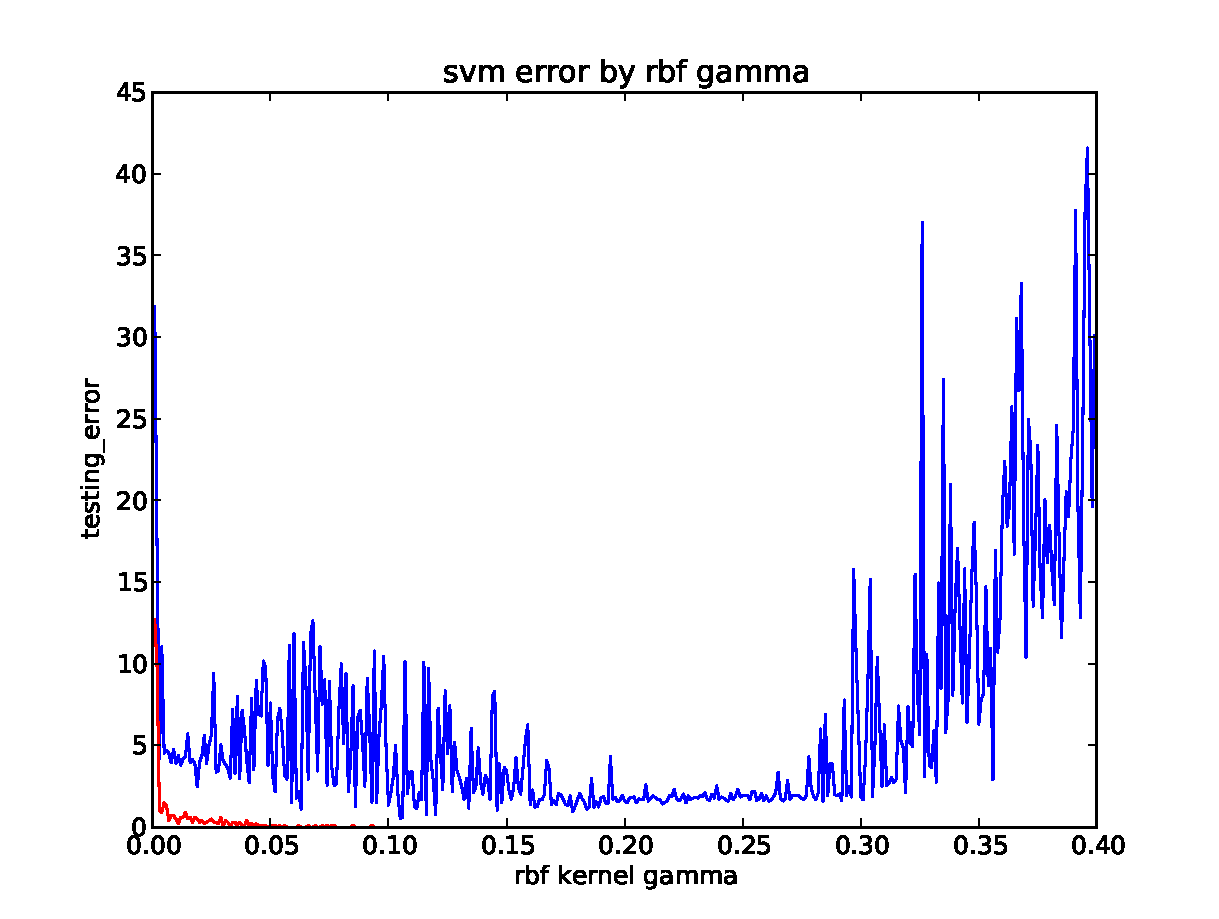
\includegraphics[width=3in]{data/agaricus-lepiota/svm/rbf.pdf}
    \caption{Mushroom - error by svm rbf gamma\label{ag-svm-rbf}}
\end{figure} 

\subsection{k-nearest neighbor}
%You should implement kNN. Use different values of k.

Initial performance results, with a single nearest neighbor, show a classification error of 3\%. Figure~\ref{ag-knn-k} shows the results of experimenting with various values for k. The plot indicates that k=3 lowered the error on a 1,000 instance training set to 2.5\%. 

\begin{figure}[!htbp]
    \centering
    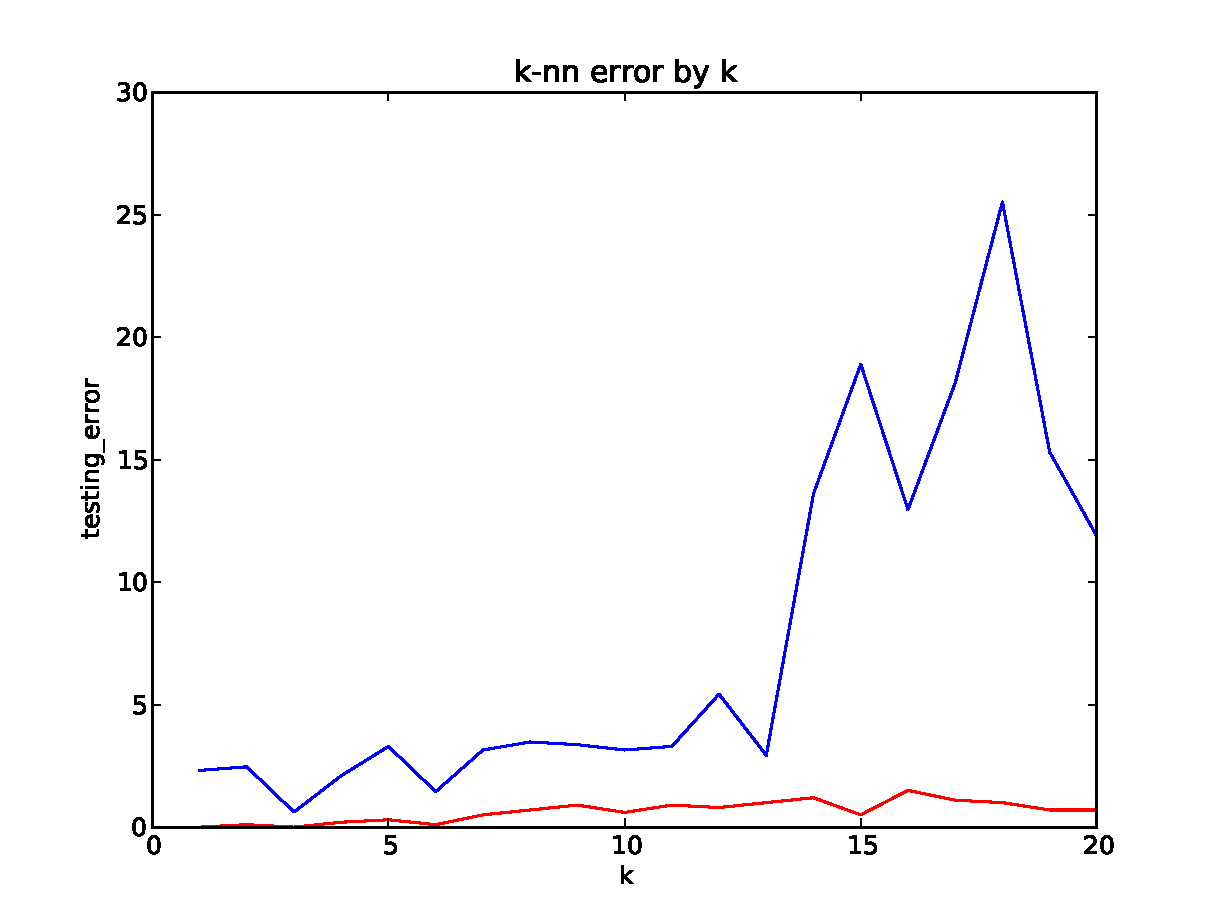
\includegraphics[width=3in]{data/agaricus-lepiota/k-nn/k.pdf}
    \caption{Mushroom - error by number of k-nn neighbors\label{ag-knn-k}}
\end{figure} 






\section{Classification - Income}

Our second dataset was also chosen from the UCI ML Repository and is titled, Adult \cite{Bache+Lichman:2013}. The classification task in this case is to determine if one's household income exceeds \$50,000/yr based on 14 biographical attributes. The data was collected from a census database from 1994. Attributes include the subject's age, level of education, marital-status, occupation, race, sex, etc. The full description of attributes can be found at http://archive.ics.uci.edu/ml/datasets/Adult.

Unlike the first classification task, this dataset is made up of both nominal and numerical attributes. This allowed comparisons between each learner's behavior with the differing profile of attribute types.

\subsection{Attribute characteristics}

Value distributions for the income dataset are shown in Figure~\ref{ad-data-viz}. In this classification task, it is not as clear as before what attributes will contribute to correct classifications. Classes are fairly evenly distributed amongst the various attribute values. Some domain knowledge could help to make intuitive judgments. For example, individuals with high capital gains or losses would suppose greater net worth, and likely greater income. Income could also correlate to one's occupation or education level.

Another difference with this dataset is that the two classes are not as evenly distributed (76\% under 50k, 24\% over 50k). This will have implications when analyzing the performance of the various learners. The chosen metric will need to conform the use cases for the resulting model. For example, if the end user is most interested in correctly identifying all individuals with incomes greater than 50k, the performance metric should be the recall for that class. As can be seen in the example accuracy results from Figure~\ref{ad-metrics}, the classifier did well at positively identifying people making under 50k (0.95 true positive rate). However, it was only able to correctly identify 55\% of those making over 50k.


\begin{figure}[!htbp]
    \centering
    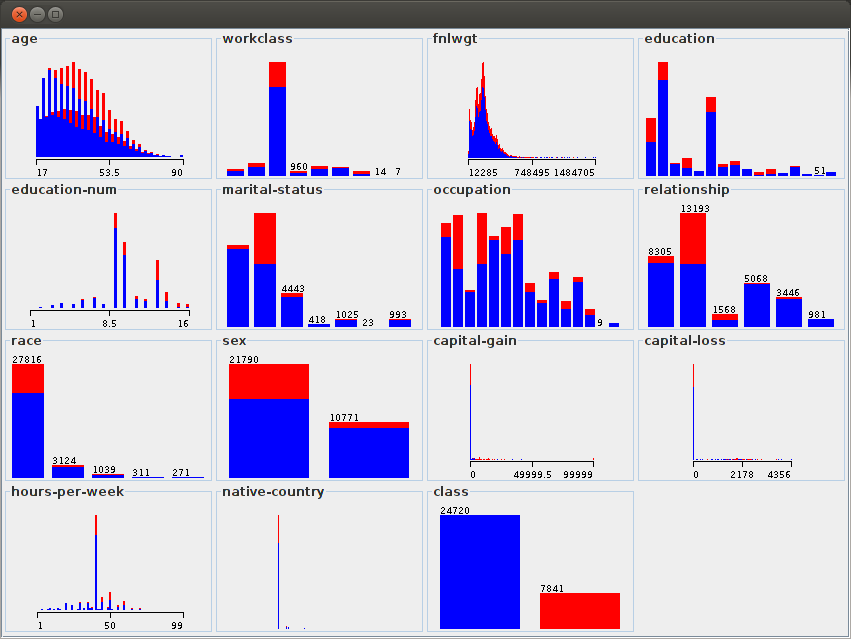
\includegraphics[width=3in]{data/adult/ad-data-viz.png}
    \caption{income attribute distribution and classification \label{ad-data-viz}}
\end{figure} 

\tiny
\begin{verbbox}
=== Detailed Accuracy By Class ===

               TP Rate   FP Rate   Precision   Recall  F-Measure   ROC Area  Class
                 0.952     0.449      0.873     0.952     0.911      0.865     <=50K
                 0.551     0.048      0.779     0.551     0.645      0.865     >50K
Weighted Avg.    0.858     0.355      0.851     0.858     0.849      0.865

=== Confusion Matrix ===

    a    b   <-- classified as
 8064  406 |    a =  <=50K
 1168 1433 |    b =  >50K
\end{verbbox}
\normalsize

\begin{figure}[!htbp]
    \centering
    \theverbbox
    \caption{example accuracy metrics for income \label{ad-metrics}}
\end{figure}


For the purposes of evaluating the current set of learners, the weighted average f-score (f-measure in Weka) was used. This provides a measure of both precision and recall metrics across both classes, thus testing each learner's ability to achieve a balanced confusion matrix.



\subsection{Algorithm Evaluations}

\subsubsection{Learning Curves}

As before, the same starting parameters were chosen for each learner. Then training was performed against a range of training set sizes (10 to 2,000 by 10). The difference in this task is that instead of using classification error as our performance metric, we will be using the weighted f-score. Figure~\ref{ad-error} shows the results of this initial experiment (blue=testing set, red=training set).

\begin{figure}[!htbp]
    \centering
    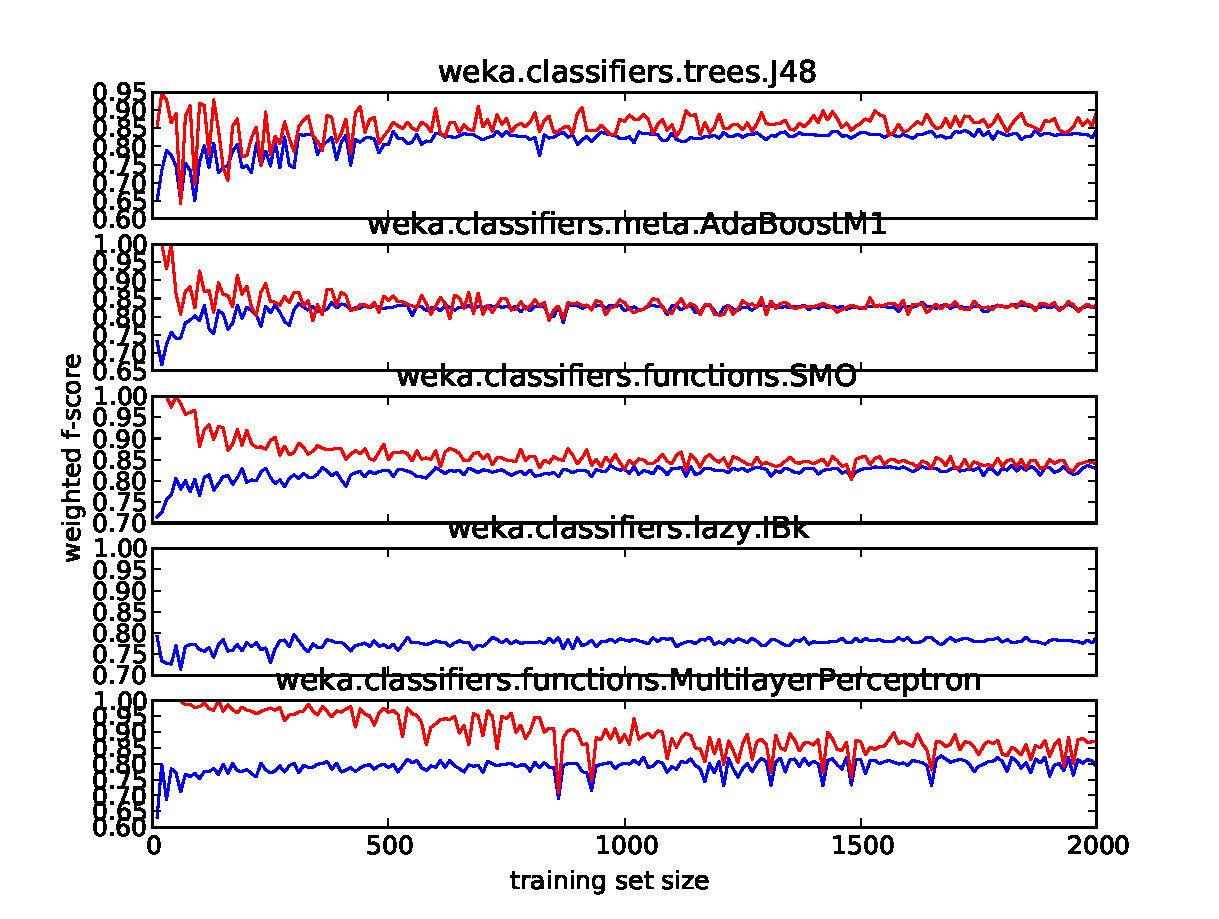
\includegraphics[width=3in]{data/adult/learning-curve-10to2000/stacked-fscore.pdf}
    \caption{Income - F-Score by Training Size \label{ad-error}}
\end{figure} 

It is interesting to observe how the f-score on the testing set begins low and raises as training instances are added, while the opposite behavior occurs with the training set f-score. This is expected behavior, as it is easier to find a hypothesis that fits a small set of training data, but does not generalize well to the test set. Conversely, it becomes more difficult to fit a larger training set and the learner is forced to find a hypothesis that generalizes better. The learner could overfit the data, in which case the training error would remain low and the testing error would eventually begin raising again. This behavior was not exhibited in the initial experiment. 


\subsubsection{Training Times}

Each learner, with naive parameters, seems to perform similarly across the training set sizes, with k-NN acheving slightly lower f-scores. However, there is a significant difference in the training times as seen in Figure~\ref{ad-runtime}. As seen in the previous classification experiment, the neural network took significantly longer to train for each training set size. In this case the difference was nearly three orders of magnitude greater than the other eager learners.

Again, k-NN did take some time to process the training set, which is believed to be attributed to sorting the instances for faster distance calculations.

\begin{figure}[!htbp]
    \centering
    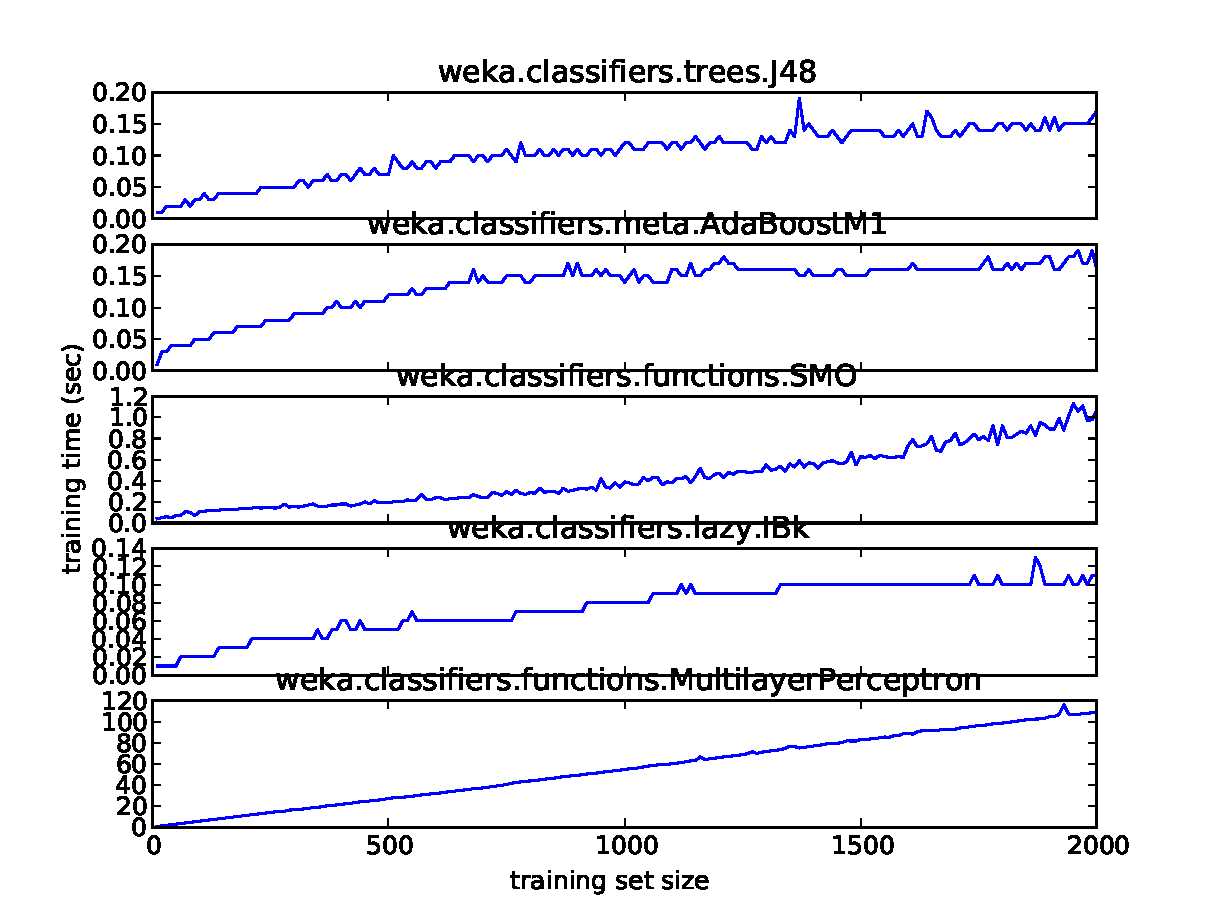
\includegraphics[width=3in]{data/adult/learning-curve-10to2000/runtime.pdf}
    \caption{Income - Training Time by Training Size \label{ad-runtime}}
\end{figure} 


\subsection{Decision Trees}
%Decision Trees. For the decision tree, you should implement or steal a decision tree algorithm. Be sure to use some form of pruning. You are not required to use information gain (for example, there is something called the GINI index that is sometimes used) to split attributes, but you should describe whatever it is that you do use.

The fact that this dataset is made up of both continuous and discrete attributes means that we must address the issue of how to split numerical attributes at decision nodes. The C4.5 algorithm, which is used in this case, is natively able to handle continuous attributes by finding a value threshold that maximizes the information gain ratio on the resulting two sets of instances.

The results of running the C4.5 decision tree algorithm on a 1,000 instance training set and a 0.25 confidence factor for post-pruning resulted in the tree shown in Figure~\ref{ad-dt-c025}. We can observe a few interesting results from this tree. First, the capital-gain attribute was chosen as the first node despite the fact that it's information gain at the first node is quite small compared to other attributes (0.08978 vs. 0.18 for relationship). This discrepancy is accounted for by examining the instances directly. We see that capital-gain has a value of 0 for most of the instances. In contrast, other attributes take on a wide range of values and thus have an unfair advantage in the information gain calculation. To compensate for this, C4.5 uses the normalized information gain ratio, which is specifically designed to account for these cases of imbalanced value distribution. Using this metric, we see that capital-gain does rank highest among the attributes (0.3 vs. 0.085 for relationship).

\small
\begin{verbbox}
capital-gain <= 5013
|   education-num <= 11
|   |   age <= 28:  <=50K (221.0/1.0)
|   |   age > 28
|   |   |   capital-loss <= 625:  <=50K (442.0/70.0)
|   |   |   capital-loss > 625
|   |   |   |   capital-loss <= 1651:  <=50K (7.0/1.0)
|   |   |   |   capital-loss > 1651:  >50K (12.0/3.0)
|   education-num > 11
|   |   marital-status =  Never-married:  <=50K (76.0/9.0)
|   |   marital-status =  Married-civ-spouse:  >50K (147.0/41.0)
|   |   marital-status =  Divorced
|   |   |   hours-per-week <= 44:  <=50K (22.0)
|   |   |   hours-per-week > 44
|   |   |   |   fnlwgt <= 112497:  >50K (4.0)
|   |   |   |   fnlwgt > 112497:  <=50K (8.0/1.0)
|   |   marital-status =  Married-spouse-absent:  <=50K (7.0/1.0)
|   |   marital-status =  Separated:  <=50K (2.0/1.0)
|   |   marital-status =  Married-AF-spouse:  <=50K (0.0)
|   |   marital-status =  Widowed:  <=50K (2.0)
capital-gain > 5013:  >50K (50.0/2.0)

Number of Leaves  :     14

Size of the tree :  22
\end{verbbox}
\normalsize

\begin{figure}[!htbp]
    \centering
    \theverbbox
    \caption{c4.5 decision tree with 0.25 confidence interval \label{ad-dt-c025}}
\end{figure}


In order to determine if the resulting tree is overfitting the data, experiments were run with varying degrees of post-pruning, including disabling pruning altogether. The results in Figure~\ref{ad-dt-pr} show us that our weighted f-score does not vary significantly with larger or smaller trees. We do see from Figures~\ref{ad-dt-sm}~and~\ref{ad-dt-lg} that recall for the greater than 50k class is better with the larger tree (0.623 vs. 0.545). It turns out that most of the under 50k classified instances are identified near the top of the tree. Adding additional nodes helps to identify more over 50k instances, but does not impact the tree's ability to classify the under 50k class.



\begin{figure}[!htbp]
    \centering
    \small
    \begin{tabular}{ | l | l | l | l | }
        \hline
        Pruned & Confidence Factor & Weighted F-Score & Tree Size\\ \hline
        no & n/a & 0.837 & 136\\ \hline
        yes & 0.25 & 0.836 & 22\\ \hline
        yes & 0.1 & 0.833 & 16\\ \hline
        yes & 0.01 & 0.834 & 12\\ \hline
    \end{tabular}
    \normalsize
    \caption{decision tree results with various levels of pruning \label{ad-dt-pr}}
\end{figure}


\tiny
\begin{verbbox}
=== Detailed Accuracy By Class ===

               TP Rate   FP Rate   Precision   Recall  F-Measure   ROC Area  Class
                 0.939     0.455      0.864     0.939     0.9        0.758     <=50K
                 0.545     0.061      0.742     0.545     0.629      0.758     >50K
Weighted Avg.    0.842     0.359      0.835     0.842     0.834      0.758

=== Confusion Matrix ===

    a    b   <-- classified as
 7851  513 |    a =  <=50K
 1231 1476 |    b =  >50K
\end{verbbox}
\normalsize

\begin{figure}[!htbp]
    \centering
    \theverbbox
    \caption{performance metrics - C4.5 - 12 node tree\label{ad-dt-sm}}
\end{figure}

\tiny
\begin{verbbox}
=== Detailed Accuracy By Class ===

               TP Rate   FP Rate   Precision   Recall  F-Measure   ROC Area  Class
                 0.91      0.377      0.882     0.91      0.896      0.857     <=50K
                 0.623     0.09       0.693     0.623     0.656      0.857     >50K
Weighted Avg.    0.84      0.307      0.836     0.84      0.837      0.857

=== Confusion Matrix ===

    a    b   <-- classified as
 7615  749 |    a =  <=50K
 1020 1687 |    b =  >50K

\end{verbbox}
\normalsize

\begin{figure}[!htbp]
    \centering
    \theverbbox
    \caption{performance metrics - C4.5 - 136 node tree\label{ad-dt-lg}}
\end{figure}



\subsection{Neural networks}
%For the neural network you should implement or steal your favorite kind of network and training algorithm. You may use networks of nodes with as many layers as you like and any activation function you see fit.

The neural network learner was again evaluated with a number of varying parameters. Our network in this case was smaller with initial settings than in the first classification task. Again a single hidden layers was created with the number of nodes totaling 1/2 the number of attributes and classifications. These settings resulted in an f-score of 0.8. Using the same training set, a network was then created with no hidden layer. The resulting f-score was 0.818. Recall and precision for each class were not greatly impacted by the inclusion or removal of the hidden layer either. To be thorough, the same experiment was performed with four nodes in a hidden layer. This produced nearly identical results to the network with no hidden layer.


As before, different learning rates and training iterations were evaluated. The results are displayed in Figures~\ref{ad-nn-ti}~and~\ref{ad-nn-lr}. The f-score by training iterations plot does not show a discernible pattern. A minimal number of training iterations allowed the learner to find a hypothesis that was just as good, according to our performance metric, as one built with many more back-propagation weight update cycles. The implication of this observation is that our neural network can be trained much faster, in terms of elapsed time. Figure~\ref{ad-nn-time} shows that if we perform 100 update cycles, the training time would be 1/5 of what was observed in the first performance experiment. This reduced training time would not significantly affect the f-score obtained for a given training set size.

\begin{figure}[!htbp]
    \centering
    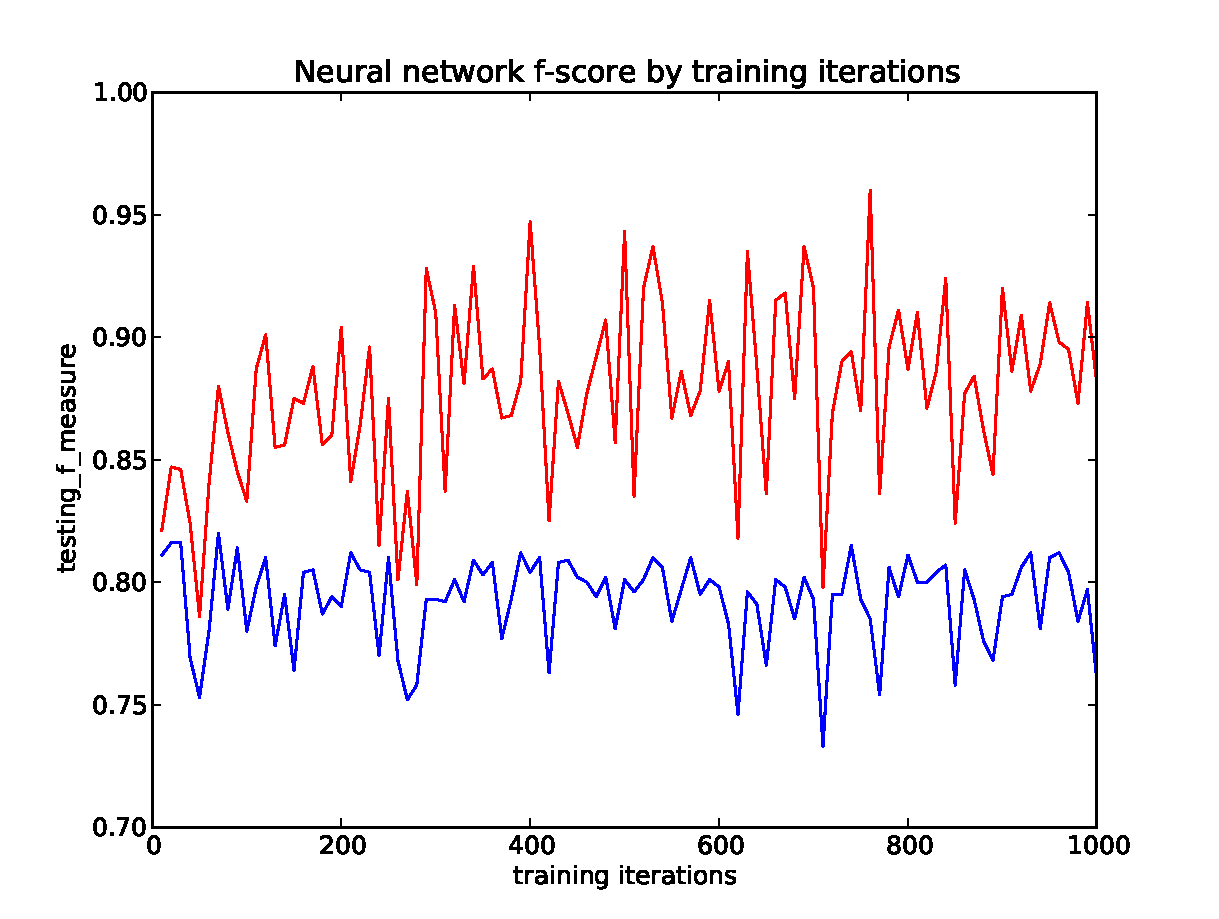
\includegraphics[width=3in]{data/adult/perceptron/training-iterations.pdf}
    \caption{income - neural network f-score by training iterations \label{ad-nn-ti}}
\end{figure} 

\begin{figure}[!htbp]
    \centering
    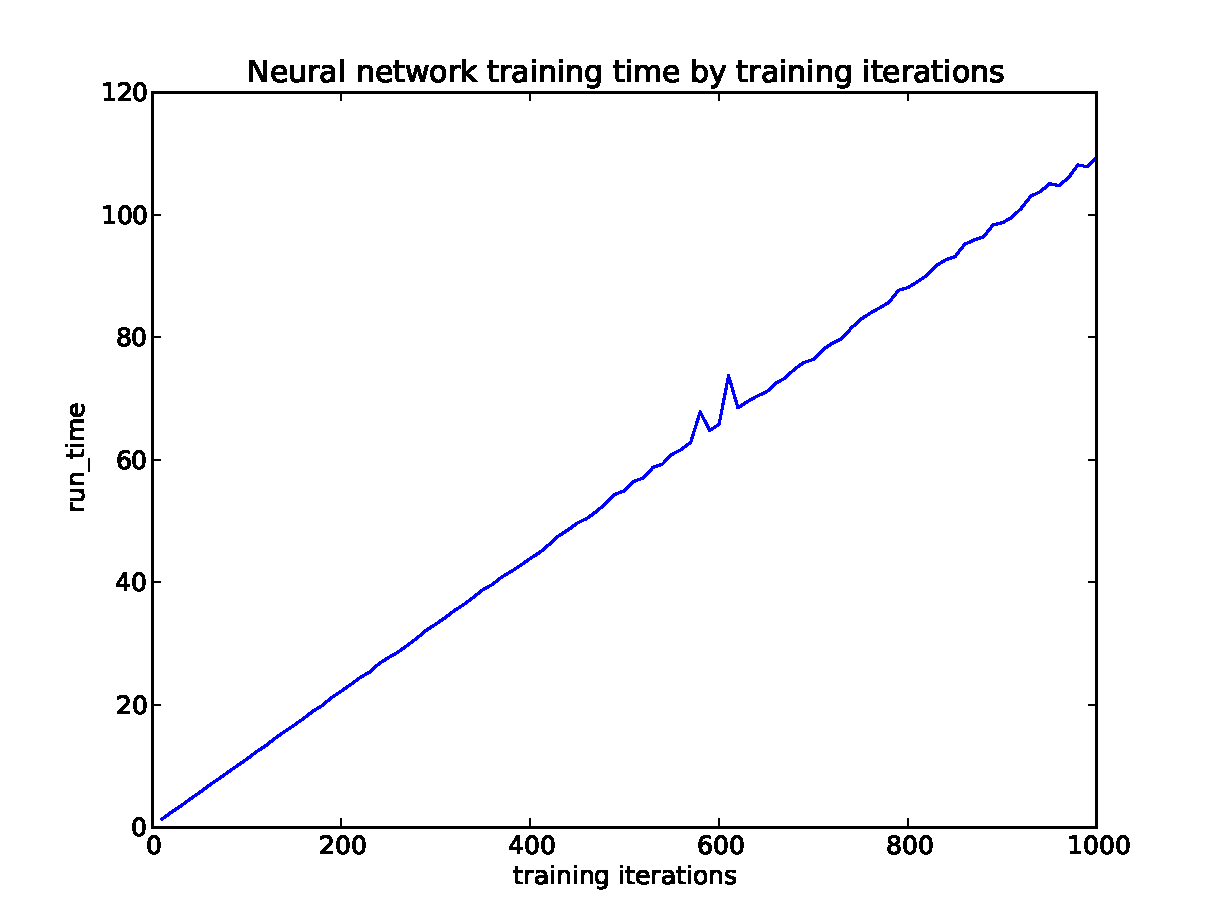
\includegraphics[width=3in]{data/adult/perceptron/time-iterations.pdf}
    \caption{income - neural network training time  by iterations \label{ad-nn-time}}
\end{figure} 


We encounter an interesting result when varying the learning rate (Figure~\ref{ad-nn-lr}). We see that more aggressive changes to the weights begins to have a negative effect on the performance of the learner. The gradient decent process seems be moving past the minimum point on each subsequent update. As the learning rate is increased further, this over-correcting behavior becomes more pronounced.


\begin{figure}[!htbp]
    \centering
    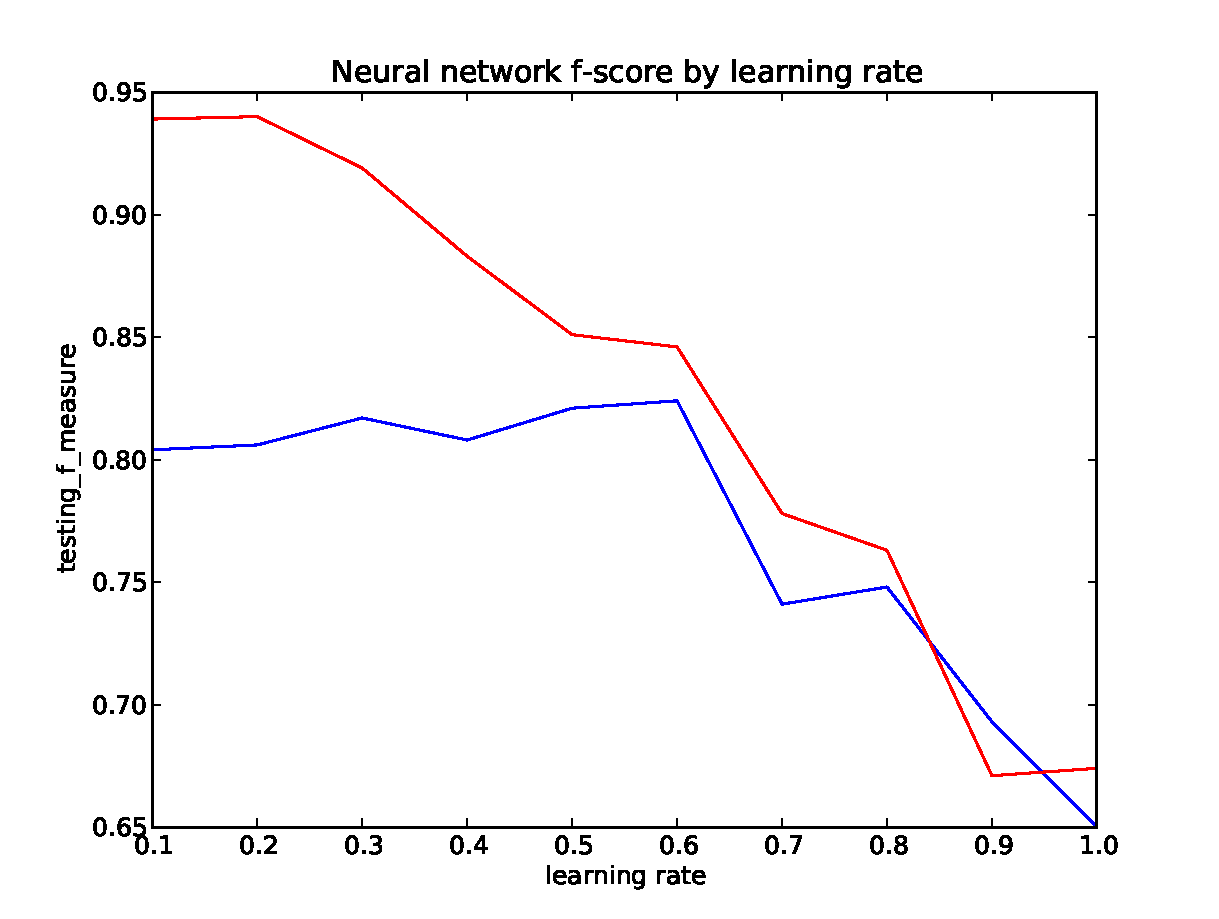
\includegraphics[width=3in]{data/adult/perceptron/learning-rate.pdf}
    \caption{income - neural network f-score by learning rate \label{ad-nn-lr}}
\end{figure} 


Figure~\ref{ad-nn-weights} shows the attributes with the most extreme weights from the output node corresponding to the over 50k classification. This is from the network trained with no hidden layer. By examining the weights in this way, we are able to identify what attributes provide the best indicators for the given class. In this example, capital-gain/loss is again shown to have a significant impact on whether a sample should be classified as over 50k. This examination would also work with tasks involving more than two classes. We should be able to construct a two layer neural network and examine the weights on the output nodes to get an intuition regarding what attributes make good indicators for any of the given classes.


\scriptsize
\begin{verbbox}
    Attrib education-num                         12.851090607340847
    Attrib education= 10th                       -14.49169769903813
    Attrib marital-status= Married-civ-spouse    11.577092459018411
    Attrib capital-gain                          16.178951592770375
    Attrib capital-loss                          13.576768257089594
    Attrib hours-per-week                        11.598543101564479
\end{verbbox}
\normalsize

\begin{figure}[!htbp]
    \centering
    \theverbbox
    \caption{neural network sample output node weights \label{ad-nn-weights}}
\end{figure}


\subsection{Boosting}
%Implement a boosted version of your decision trees. As before, you will want to use some form of pruning, but presumably because you're using boosting you can afford to be much more aggressive about your pruning.

Boosting performed quite well on the initial performance experiment. The learner was able to reach high f-score numbers with a limited training set size. Boosting iterations were again varied to examine the impact to the learner's performance (Figure~\ref{ad-boost-iter}). Unlike the mushroom classification task, adding boosting iterations in this case had no noticeable degradation in performance. The previous result was attributed to overfitting and the fact that most of the classification accuracy was derived from a single attribute. On the income dataset, it seems that the more subtle relationships between the attributes and classes prevents our boosted learner from overfitting the data.

\begin{figure}[!htbp]
    \centering
    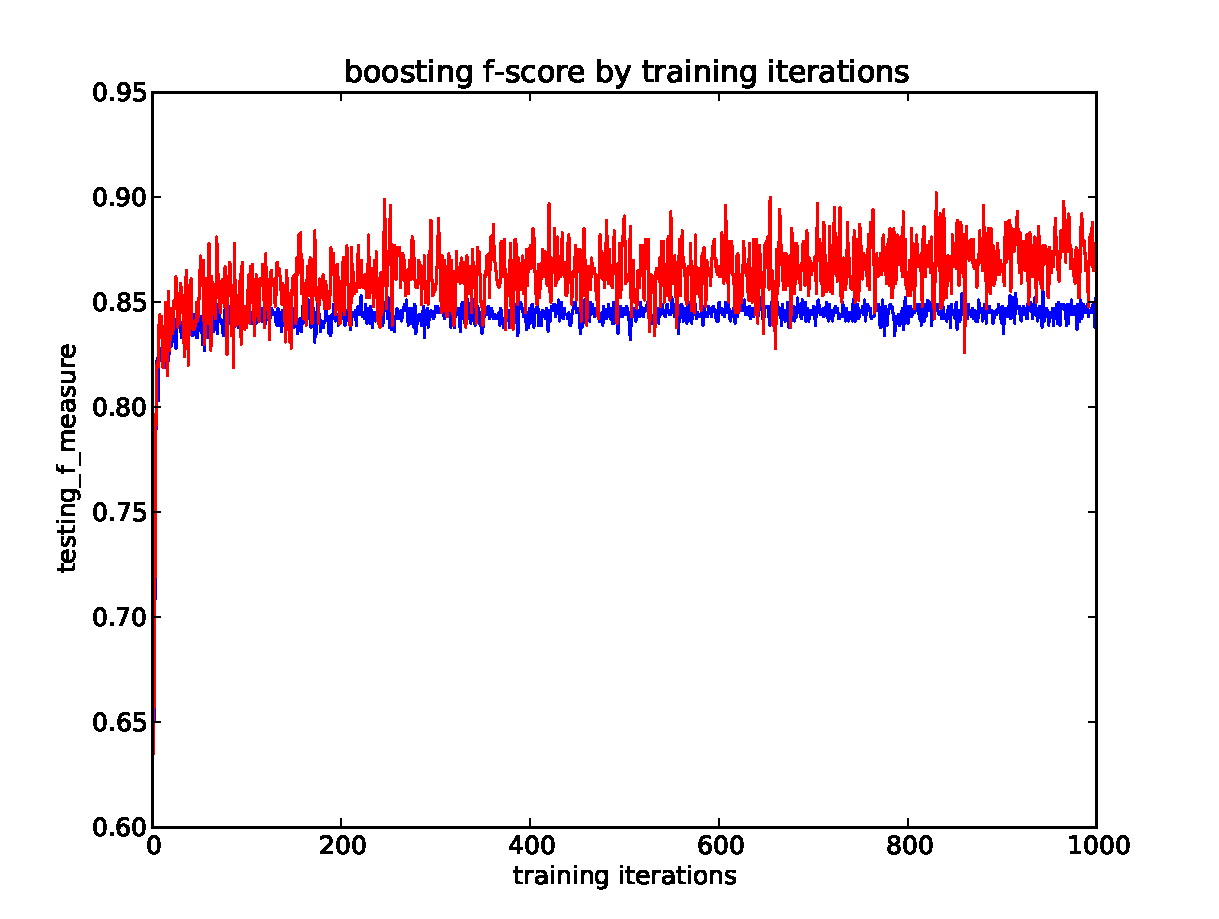
\includegraphics[width=3in]{data/adult/boosting/training-iterations.pdf}
    \caption{income - f-score by boosting iterations \label{ad-boost-iter}}
\end{figure} 

In order to throughly examine the options for this learner, the original experiment was conducted with C4.5 as the boosted classifier. The post-pruning parameters were also varied to allow for more generalized trees. In each of these experiments, the performance numbers did not significant improve from our original classifier (decision stump).


\subsection{Support Vector Machines}
%You should implement (for sufficently loose definitions of implement including download) SVMs. This should be done in such a way that you can swap out kernel functions. I'd like to see at least two.

SVM performance for this classification task was similar to that of the previous experiments. As seen before, the learner was able to reach good f-score numbers with a reasonably small training set. Also as expected, training time was between that of the decision tree and neural network learners. Although the neural network was vastly slower than the others. Changes were again made to the SVM polynomial kernel to see if higher dimensional mappings would help improve the linear separability of the dataset. Figure~\ref{ad-svm-poly} shows that the greatest f-score was achieved with a linear kernel, which was a very different result than what was seen with the previous dataset.

\begin{figure}[!htbp]
    \centering
    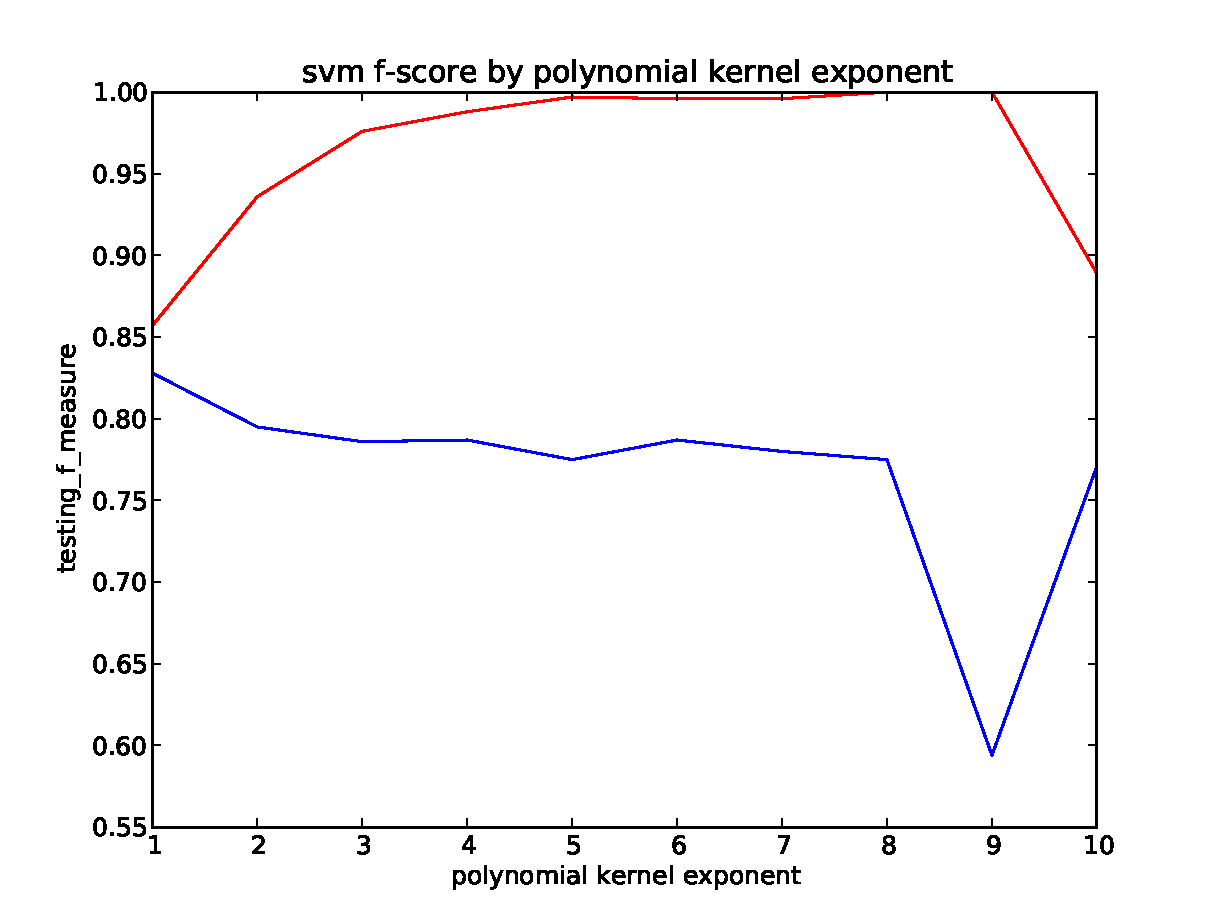
\includegraphics[width=3in]{data/adult/svm/polynomial.pdf}
    \caption{income - f-score by svm polynomial kernel exponent \label{ad-svm-poly}}
\end{figure} 

Using the radial basis kernel, we can see from Figure~\ref{ad-svm-rbf} that the f-score seems to improve with a gamma around 0.03 and remains steady with higher gamma values. Between the various kernel functions, the linear kernel performed the best on the income dataset (0.83). The polynomial and RBF kernels did not do as well to separate the instances.

\begin{figure}[!htbp]
    \centering
    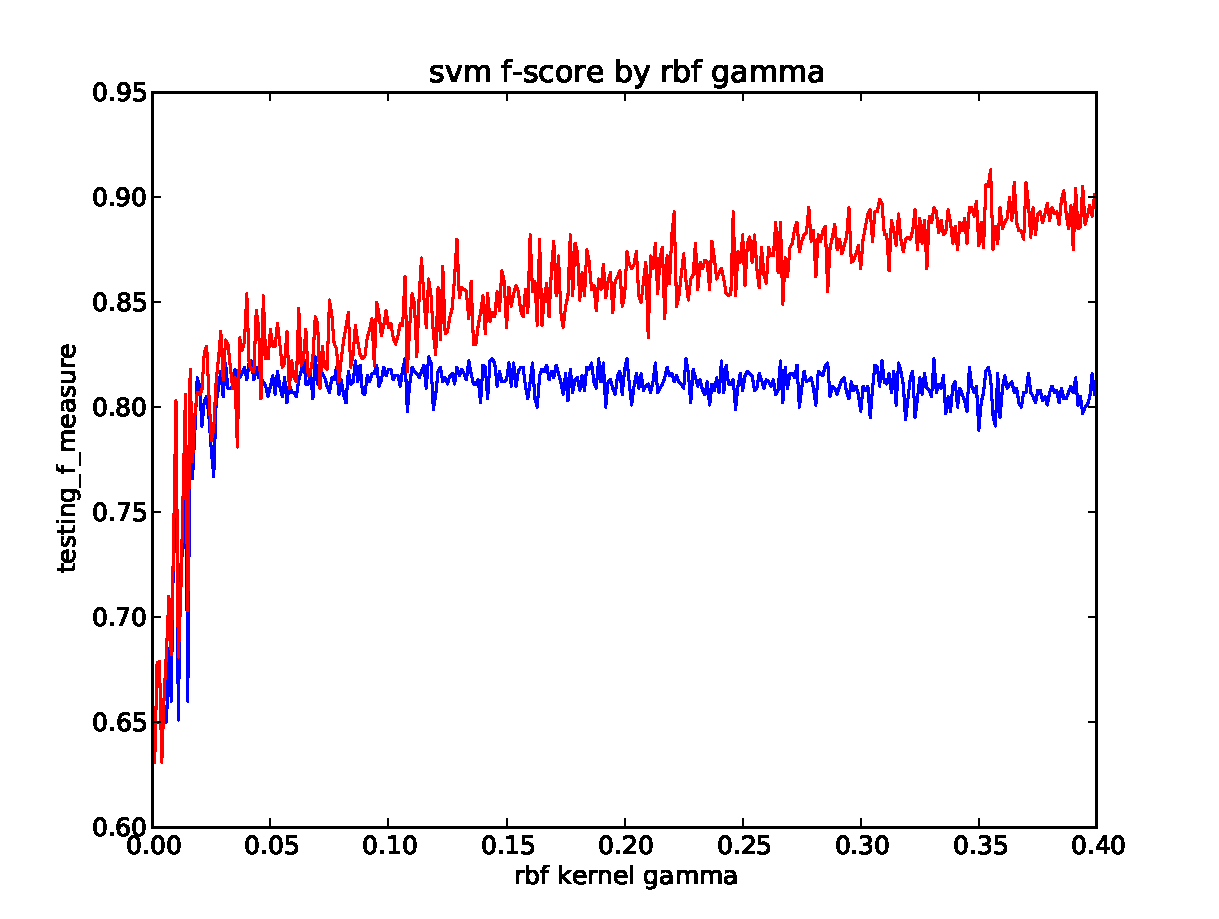
\includegraphics[width=3in]{data/adult/svm/rbf.pdf}
    \caption{income - f-score by svm rbf gamma\label{ad-svm-rbf}}
\end{figure} 

\subsection{k-nearest neighbor}
%You should implement kNN. Use different values of k.

Figure~\ref{ad-knn-k} shows an interesting result regarding the various values for k in the nearest neighbor learner. Quite unlike it's behavior on the previous dataset, this learner seemed to handle increasing number of neighbors without any significant change to the learner's performance. It also appears that k values below 10 degraded the performance of the learner.


\begin{figure}[!htbp]
    \centering
    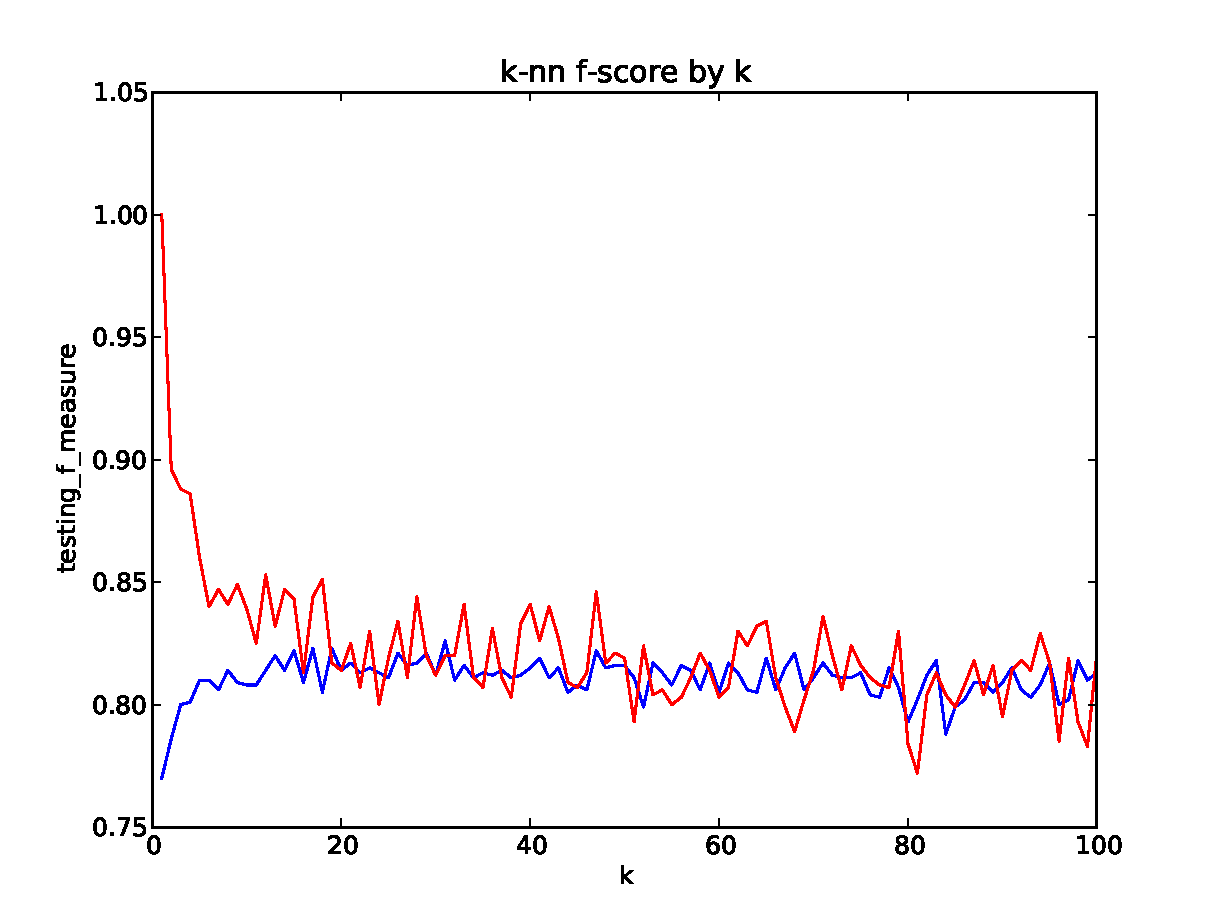
\includegraphics[width=3in]{data/adult/k-nn/k.pdf}
    \caption{income - f-score by number of k-nn neighbors\label{ad-knn-k}}
\end{figure} 



\section{Concluding Remarks}

Having explored the various facets of these two classification tasks, we see that each machine learning algorithm provides a different perspective from which to understand the relationships between the datasets' attributes and classes. Decision trees create an tangible view of how instances can be categorized by a hierarchical set of attributes evaluations. Neural networks, although they can become incomprehensible, provide an understanding of the relative importance of attributes to the classification task. SVM, and particularly the kernels involved, give us insight into the complexity of the dataset and how intermingled the classes are in the feature space. Finally, k-NN provides an human understanding of how instances are grouped by using metrics that are intuitive and commonplace.

We have seen how differently each of the learners behave from one classification task to the next. We have also explored the differences that arise in measuring an algorithm's performance, and how the end use case cannot be separated from the decisions made in approaching the learning task. Considerations as simple as how long should we train and how much data should we provide the learner can make a significant difference. We have seen that these learning tasks cannot be approached purely programmatically, and that a fair amount of judgment and interpretation is involved.




\bibliographystyle{abbrv}
\bibliography{term-paper}
\begin{thebibliography}{10}

\bibitem{Bache+Lichman:2013}
K. Bache and M. Lichman
\newblock UCI Machine Learning Repository
\newblock 2013
\newblock http://archive.ics.uci.edu/ml
\newblock University of California, Irvine, School of Information and Computer Sciences

%\bibitem{Zhong:Osteo}
%L.~Zhong, D.~El-Daye, B.~Kaufman, N.~Tobaoda, T.~Mohamed, and M.~Liebschner.
%\newblock Osteoconduct: Wireless body-area communication based on bone
  %conduction.
%\newblock In {\em in Proc. Int. Conf. Body Area Networks (BodyNets)}, June
  %2007.

\end{thebibliography}
\end{document}
